\chapter{$\Upsilon$ production in Pb+Pb collisions}
\label{chap:UpsilonProductionPbPb}

\section{$\Upsilon(nS)$ in Pb+Pb collisions}
At large energy densities and high temperatures, strongly interacting
matter consists of a deconfined and chirally-symmetric system of
quarks and gluons~\cite{Karsch:2003jg}. This state, often referred to
as ``quark-gluon plasma'' (QGP)~\cite{Shuryak:1977ut}, constitutes the
main object of the studies performed with relativistic heavy-ion
collisions~\cite{Arsene:2004fa,Back:2004je,Adcox:2004mh,Adams:2005dq}.

The formation of a QGP in high-energy nuclear collisions can be
evidenced in a variety of ways. One of its most striking expected
signatures is the suppression of quarkonium
states~\cite{SATZ}, both of the charmonium (\Jpsi, $\psi'$,
$\chi_c$, etc.) and the bottomonium ($\PgU\text{(1S,\,2S,\,3S)}$,
$\chi_b$, etc.) families.  This is thought to be a direct effect of
deconfinement, when the binding potential between the constituents of
a quarkonium state, a heavy quark and its antiquark, is screened by
the colour charges of the surrounding light quarks and gluons.  The
suppression is predicted to occur above the critical temperature of
the medium ($T_c$) and depends on the \QQbar binding energy. Since the
\PgUa\ is the most tightly bound state among all quarkonia, it is
expected to be the one with the highest dissociation
temperature. Examples of dissociation temperatures are given in
Ref.~\cite{Mocsy:2007jz}: $T_{\text{dissoc}}\sim\!1\,T_c$, $1.2\,T_c,$
and $2\,T_c$ for the \PgUc, \PgUb, and \PgUa, respectively. Similarly,
in the charmonium family the dissociation temperatures are
$\leq1\,T_c$ and $1.2\,T_c$ for the $\psi'$ and \Jpsi,
respectively. However, there are further possible changes to the
quarkonium production in heavy-ion collisions. On the one hand,
modifications to the parton distribution functions inside the nucleus
(shadowing) and other cold-nuclear-matter effects can reduce the
production of quarkonia without the presence of a
QGP~\cite{Vogt:2010aa,Zhao:2011cv}. On the other hand, the large
number of heavy quarks produced in heavy-ion collisions, in particular
at the energies accessible by the Large Hadron Collider (LHC), could
lead to an increased production of quarkonia via statistical
recombination~\cite{Zhao:2010nk,Andronic:2006ky,Capella:2007jv,Thews:2005vj,Yan:2006ve,Grandchamp:2005yw}.

Charmonium studies in heavy-ion collisions have been carried out for
25 years, first at the Super Proton Synchrotron (SPS) by the
NA38~\cite{Baglin:1994ui},
NA50~\cite{Alessandro:2004ap,Alessandro:2006ju}, and
NA60~\cite{Arnaldi:2007zz} fixed-target experiments at 17.3--19.3\GeV
centre-of-mass energy per nucleon pair (\sqrtsnn), and then at the
Relativistic Heavy Ion Collider (RHIC) by the PHENIX experiment at
\sqrtsnn = 200\GeV~\cite{Adare:2006ns}. In all cases, \Jpsi
suppression was observed in the most central collisions. At the SPS,
the suppression of the $\psi'$ meson was also
measured~\cite{Alessandro:2006ju}. Experimentally, the suppression is
quantified by the ratio of the yield measured in heavy-ion collisions
and a reference. At RHIC, the reference was provided by the properly
scaled yield measured in \pp collisions. Such a ratio is called the
nuclear modification factor, \raa. In the absence of modifications,
one would expect \raa = 1 for hard processes, which scale with the
number of inelastic nucleon-nucleon collisions. For bottomonia, the
production cross section is too small at RHIC to make definitive
statements~\cite{Abelev:2010am}. With the higher energy and luminosity
available at the LHC, new studies for charmonia and bottomonia have
become possible. 

\section{Data Selection}
\label{sec:data-selection}
\subsection{Event Selection}
\label{sec:event-sel}

Inelastic hadronic \PbPb collisions are selected using information
from the BSC and HF calorimeters, in coincidence with a bunch crossing
identified by the beam pick-up (one on each side of the interaction
point)~\cite{Adolphi:2008zzk}.  Events are further filtered offline by
requiring a reconstructed primary vertex based on at least two tracks,
and at least 3 towers on each HF with an energy deposit of more than
3\GeV per tower. These criteria reduce contributions from single-beam
interactions with the environment (e.g. beam-gas collisions and
collisions of the beam halo with the beam pipe), ultra-peripheral
electromagnetic interactions, and cosmic-ray muons. A small fraction
of the most peripheral PbPb collisions are not selected by these
\emph{minimum-bias} requirements, which accept $(97\pm3)$\% of the
inelastic hadronic cross section~\cite{Chatrchyan:2011sx}. A sample
corresponding to 55.7 M minimum-bias events passes all these
filters. Assuming an inelastic \PbPb cross section of $\sigma_{\PbPb}
= 7.65$~b~\cite{Chatrchyan:2011sx}, this sample corresponds to an
integrated luminosity of $\int L = 7.28\mubinv$. This
value is only mentioned for illustration purposes; the final results
are normalized to the number of minimum-bias events.

The measurements reported here are based on dimuon events triggered by
the L1 trigger, a hardware-based trigger that uses information
from the muon detectors. The CMS detector is also equipped with a
software-based high-level trigger (HLT). However, no further
requirements at the HLT level have been applied to the L1 muon objects
used for this analysis.

The event centrality distribution of minimum-bias events is compared
to events selected by the double-muon trigger in
\fig{fig:centrality}. The centrality variable is defined as the
fraction of the total cross section, starting at 0\% for the most
central collisions. This fraction is determined from the distribution
of total energy measured in both HF
calorimeters~\cite{Chatrchyan:2011pb}. Using a Glauber-model
calculation as described in Ref.~\cite{Chatrchyan:2011sx}, one can
estimate variables related to the centrality, such as the number of
nucleons participating in the collisions (\npart) and the nuclear
overlap function (\taa), which is equal to the number of elementary
nucleon-nucleon (NN) binary collisions divided by the elementary NN
cross section and can be interpreted as the NN equivalent integrated
luminosity per heavy ion collision, at a given
centrality~\cite{Miller:2007ri}. The values of these variables are
presented in \tab{tab:glauber} for the centrality bins used in this
analysis. The double-muon-triggered events are more frequent in
central collisions since the main physics processes that generate
high-p$_T$ muon pairs scale with the number of inelastic nucleon-nucleon
collisions. In the following, \npart will be the variable used to show
the centrality dependence of the measurements.

\begin{figure}[hbtp]
  \begin{center}
   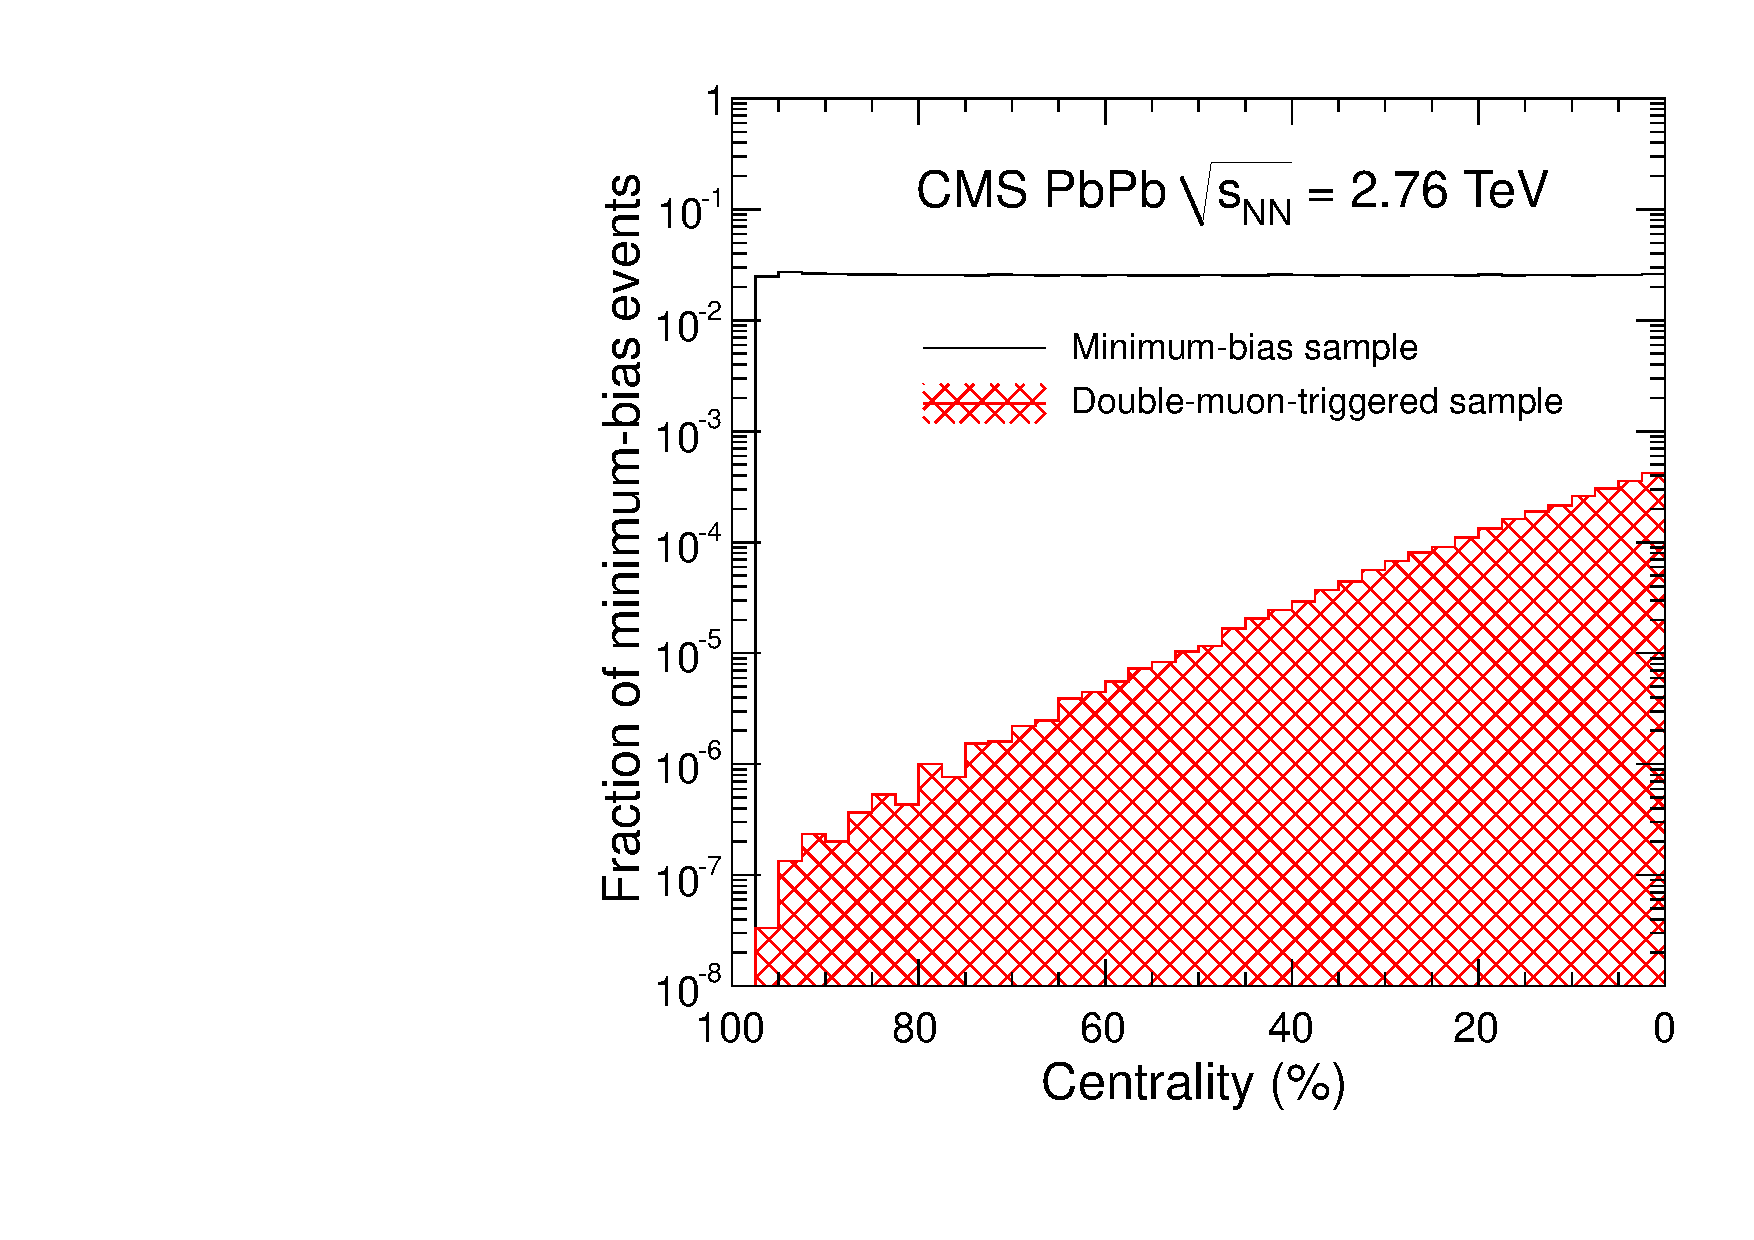
\includegraphics[width=0.5\linewidth]{chap_YInPbPbColl2010_figures/centralityDoubleMuOpen}
   \caption{Centrality distribution of the minimum-bias sample (solid
     black line) overlaid with the double-muon triggered sample
     (hashed red) in bins of 2.5\%.}
   \label{fig:centrality}
  \end{center}
\end{figure}




\begin{table}[htbp]
  \begin{center}
    \caption{Average and root-mean-square (RMS) values of the number of
      participating nucleons (\npart) and of the nuclear overlap function
      (\taa) for the centrality bins used in this
      analysis~\cite{Chatrchyan:2011sx}.}
    \label{tab:glauber}
    \begin{tabular}{rr@{.}lr@{.}lr@{.}lr@{.}lr@{.}lr@{.}lr@{.}lr@{.}l}
      \hline\vspace{0.1em}
      ~ & \multicolumn{4}{c}{$\npart$} &
      \multicolumn{4}{c}{$\taa$ (mb$^{-1}$)}\\
      Centrality (\%) & \multicolumn{2}{c}{Mean} & \multicolumn{2}{c}{RMS} & \multicolumn{2}{c}{Mean} & \multicolumn{2}{c}{RMS} \\\hline
      0--10	& 355&4 & 33&3 & 23&19 & 3&77 \\
      10--20	& 261&4 & 30&4 & 14&48 & 2&86 \\
      20--30	& 187&2 & 23&4 & 8&78  & 1&94 \\
      30--40	& 130&0 & 17&9 & 5&09  & 1&27 \\
      40--50	& 86&3  & 13&6 & 2&75  & 0&80 \\
      50--100	& 22&1  & 19&3 & 0&47  & 0&54 \\\hline
      0--20	& 308&4 & 56&8 & 18&83 & 5&49 \\
      20--100	& 64&2  & 63&0 & 2&37  & 3&05 \\\hline
      0--100	& 113&1 &115&6 & 5&66  & 7&54 \\\hline
    \end{tabular}
  \end{center}
\end{table}

\PgUa
Simulated MC events are used to tune the muon selection criteria, to
compute the acceptance and efficiency corrections, and to obtain
templates of the decay length distribution of \Jpsi from b-hadron
decays.  For the acceptance corrections described in
Section~\ref{sec:acc}, three separate MC samples, generated over full
phase space, are used: prompt J/$\psi$, J/$\psi$ from b-hadron decays,
and \PgUa. Prompt \Jpsi and \PgUa  are produced using PYTHIA
6.424~\cite{Sjostrand:2006za} at \sqrts = 2.76\TeV, which generates
events based on the leading-order colour-singlet and colour-octet
mechanisms, with non-relativistic quantum chromodynamics (QCD) matrix
elements tuned~\cite{Bargiotti:2007zz} by comparison with CDF data
~\cite{Acosta:2004yw}. The colour-octet states undergo a shower
evolution. For the non-prompt \Jpsi studies, the b-hadron events
are produced with PYTHIA in generic QCD 2$\rightarrow$2 processes. In
all three samples, the \Jpsi or \PgUa\ decay is simulated using the
EVTGEN~\cite{Lange:2001uf} package. Prompt \Jpsi and \PgUa\ are
simulated assuming unpolarized production, while the non-prompt \Jpsi
polarization is determined by the sum of the exclusive states
generated by EVTGEN. Final-state bremsstrahlung is implemented using
PHOTOS~\cite{Barberio:1993qi}.

For some MC simulation studies, in particular the efficiency
corrections described in Section~\ref{sec:eff}, the detector response
to each PYTHIA signal event is simulated with
GEANT-4~\cite{Agostinelli:2002hh} and then embedded in a realistic
heavy-ion background event. The background events are produced with
the HYDJET event generator~\cite{Lokhtin:2005px} and then simulated
with GEANT-4 as well. The HYDJET parameters were tuned to
reproduce the particle multiplicities at all centralities seen in
data. The embedding is done at the level of detector hits and requires
that the signal and background production vertices match. The embedded
event is then processed through the trigger emulation and the full
event reconstruction chain. Collision data are used to validate the
efficiencies evaluated using MC simulations, as discussed in
Section~\ref{sec:eff}.

\subsection{Muon Selection}
\label{sec:muon-sel}

The muon offline reconstruction algorithm starts by reconstructing
tracks in the muon detectors, called \emph{standalone muons}. These
tracks are then matched to tracks reconstructed in the silicon tracker
by means of an algorithm optimized for the heavy-ion
environment~\cite{D'Enterria:2007xr,Roland:2006kz}. The final muon
objects, called \emph{global muons}, result from a global fit of the
standalone muon and tracker tracks. These are used to obtain the
results presented in this paper.

In \fig{fig:muPtEtaDoable}, the single-muon reconstruction efficiency
from MC simulations is presented as a function of the muon $\pt^\mu$
and $\eta^{\mu}$. The reconstruction efficiency is defined as the
number of all reconstructed global muons divided by the number of
generated muons in a given ($\eta^{\mu}$, $\pt^{\mu}$) bin. It takes
into account detector resolution effects, i.e. reconstructed \pt and
$\eta$ values are used in the numerator and generated \pt and $\eta$
values in the denominator. To obtain a clear separation between
acceptance and efficiency corrections, a \emph{detectable} single-muon
acceptance is defined in the ($\eta^{\mu}$, $\pt^{\mu}$) space. For
the \Jpsi analysis this separation is defined by the contour that
roughly matches a global muon reconstruction efficiency of 10\%,
indicated by the white lines superimposed in \fig{fig:muPtEtaDoable},
which are described by the conditions
  
\begin{align}\label{eq:singleMuonAcc}
    \pt^{\mu} &> 3.4\GeVc &\text{ for } |\eta^{\mu}| < 1.0, \notag\\
    \pt^{\mu} &> (5.8 - 2.4\times|\eta^{\mu}|)\GeVc &\text{ for } 1.0 < |\eta^{\mu}| < 1.5,\\
    \pt^{\mu} &> (3.4 - 0.78\times|\eta^{\mu}|)\GeVc &\text{ for } 1.5 < |\eta^{\mu}| < 2.4. \notag
  \end{align}
Muons failing these conditions are accounted for in the acceptance
corrections discussed in Section~\ref{sec:acc}. Muons that pass this
acceptance requirement can still fail to pass the trigger, track
reconstruction, or muon selection requirements. These losses are
accounted for by the efficiency corrections discussed in
Section~\ref{sec:eff}.
\begin{figure}[htbp]
  \centering
  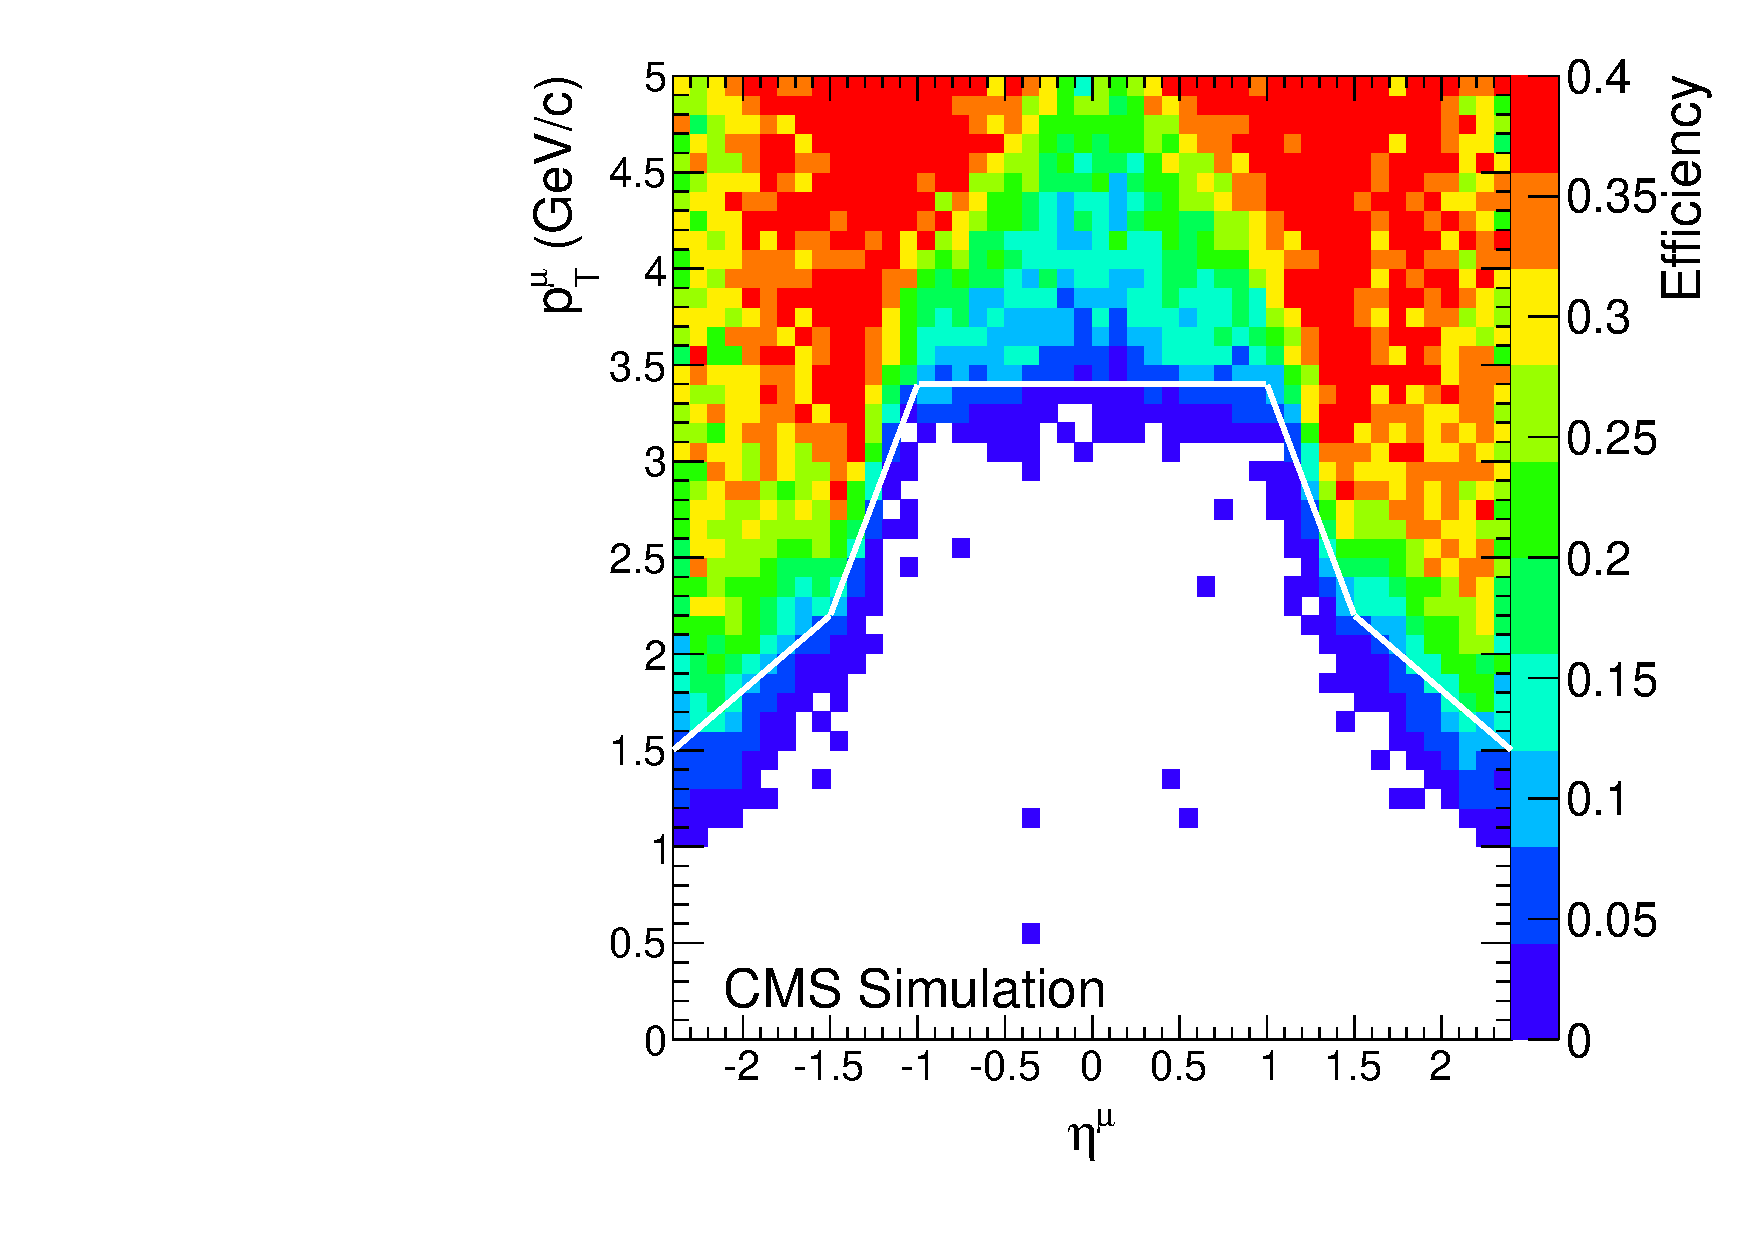
\includegraphics[width=0.5\linewidth]{chap_YInPbPbColl2010_figures/muPtEtaDoable}
  \caption{Reconstruction efficiency of global muons in the ($\eta^{\mu}$,
    $\pt^{\mu}$) space, illustrating the lower limits (white lines) of
    what is considered a detectable single muon for the analysis.}
  \label{fig:muPtEtaDoable}
\end{figure}

For the \PgUa\ analysis, where the signal-to-background ratio is less
favourable than in the \Jpsi mass range, a higher $\pt^{\mu}$ is
required than for the \Jpsi analysis,
\begin{equation}
  \label{eq:singleMuonAccUps}
    \pt^{\mu}>4\GeVc,
\end{equation}
independent of $\eta^{\mu}$.

Various additional global muon selection criteria are studied in MC
simulations. The MC distributions of the \Jpsi decay muons are in
agreement with those from data to better than 2\%, which is within the
systematic uncertainty of the data/MC efficiency ratio
(Section~\ref{sec:eff}). The transverse (longitudinal) distance of
closest approach to the measured vertex is required to be less than 3
(15)\,cm. Tracks are only kept if they have 11 or more hits in the
silicon tracker, and the $\chi^2$ per degree of freedom of the global
(inner) track fit is less than 20 (4). The $\chi^2$ probability of the
two tracks originating from a common vertex is required to be larger
than 1\%. From MC simulations we find that these criteria result in a
3.9\% loss of \PgUa\ events, respectively, given two reconstructed 
tracks associated with the double muon trigger.

\section{Signal Extraction}
\label{sec:signal-extraction}
\subsection{\texorpdfstring{\PgUa}{Upsilon(1S)} Analysis}
\label{sec:upsilon}
To extract the \PgUa\ yield, an extended unbinned maximum-likelihood
fit to the \mumu invariant mass spectrum between 7 and 14 GeV/$c^2$ is
performed, integrated over \pt, rapidity, and centrality, as shown in
the left panel of \fig{fig:ups_invmass}. The measured mass line shape
of each \PgU\ state is parametrised by a Crystal Ball function. Since
the three \PgU\ resonances partially overlap in the measured dimuon
mass spectrum, they are fitted simultaneously. Therefore, the
probability distribution function describing the signal consists of
three Crystal Ball functions. In addition to the three \PgUn\ yields,
the \PgUa\ mass is the only parameter left free, to accommodate a
possible bias in the momentum scale calibration. The mass ratios
between the states are fixed to their world average
values~\cite{Nakamura:2010zzi}, and the mass resolution is forced to
scale linearly with the resonance mass. The \PgUa\ resolution is fixed
to the value found in the simulation, 92 MeV/$c^2$. This value is
consistent with what is measured when leaving this parameter free in a
fit to the data, $(122 \pm 30) MeV/c^2$. The low-side tail parameters in
the Crystal Ball function are also fixed to the values obtained from
simulation. Finally, a second-order polynomial is chosen to describe
the background in the mass range 7--14 GeV/$c^2$. From this fit, before
accounting for acceptance and efficiencies, the measured \PgUa\ raw
yield is $86 \pm 12$. The observed suppression of the excited states
was discussed in~\cite{Chatrchyan:2011pe}. The fitted mean value is
$m_0 = (9.441\pm0.016) GeV/c^2$, which is, slightly below the PDG 
value $m_{\PgUa} = 9.460 GeV/c^2$~\cite{Nakamura:2010zzi} because
of slight momentum scale biases in the data reconstruction.

\begin{figure*}[htbp]
  \begin{center}
    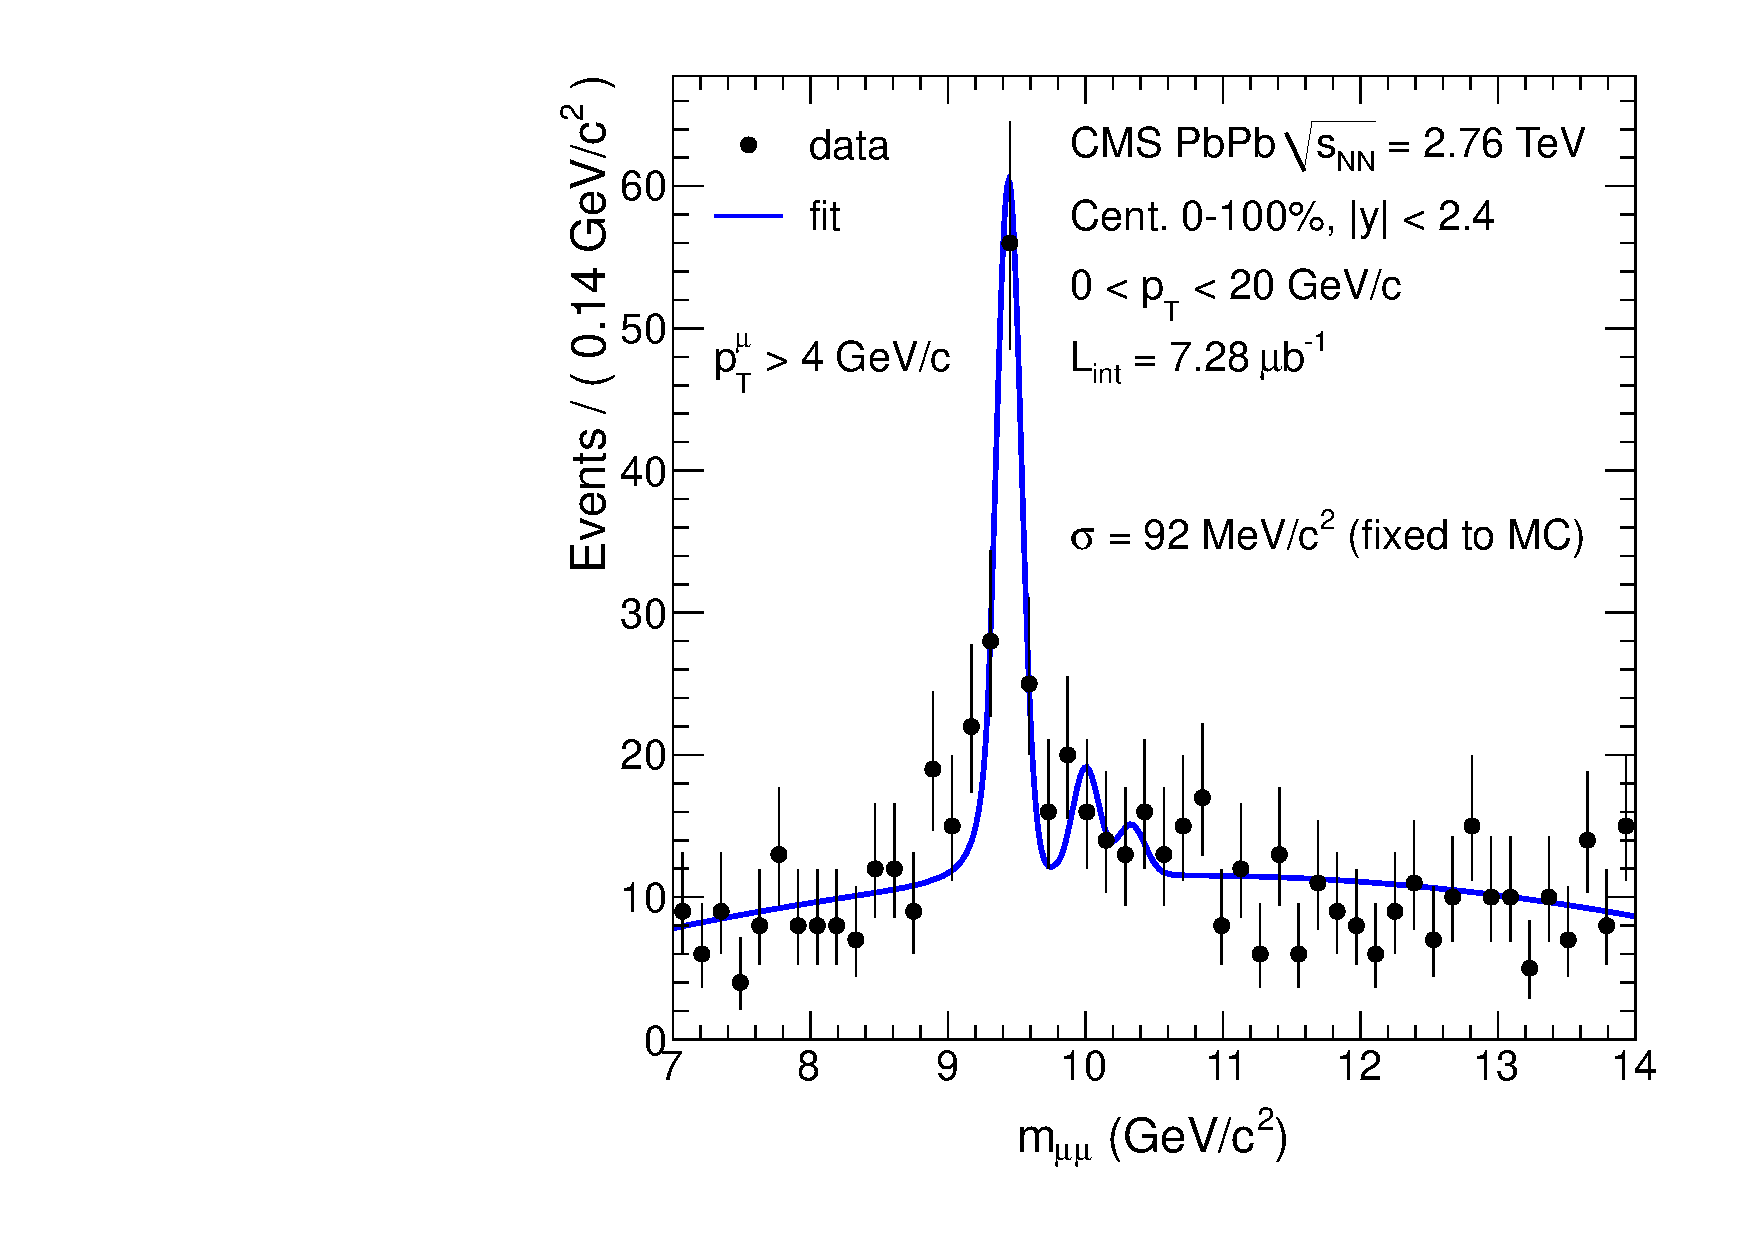
\includegraphics[width=0.45\textwidth]{chap_YInPbPbColl2010_figures/masspeak_Hi.pdf}
    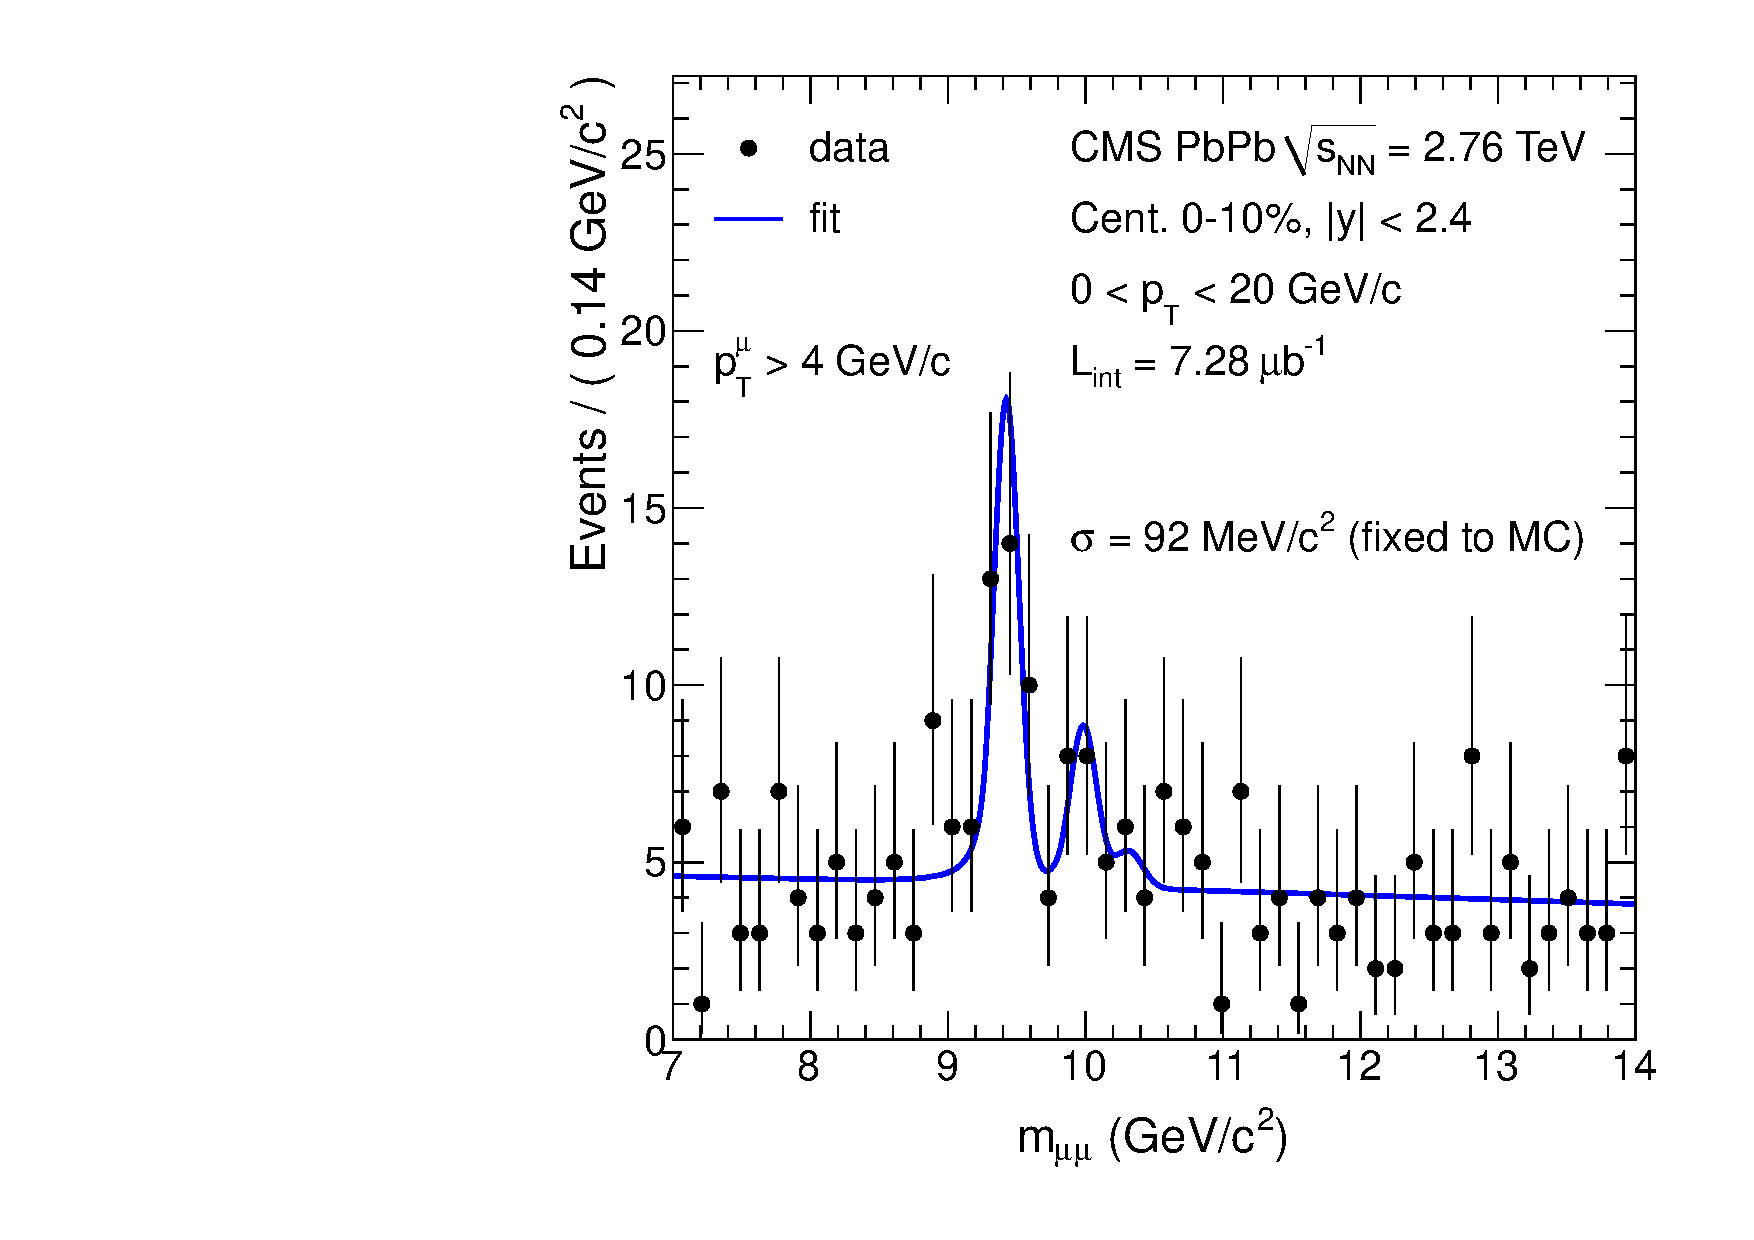
\includegraphics[width=0.45\textwidth]{chap_YInPbPbColl2010_figures/masspeak_Hi_cntr0-10.pdf}
    \caption{Invariant-mass spectrum of \mumu pairs (black circles)
      with $\pt<20\GeV/c$ and $|y|<2.4$, for muons above 4\GeVc,
      integrated over centrality (left) and for the 0--10\% centrality
      bin (right).}
    \label{fig:ups_invmass}
  \end{center}
\end{figure*}

The data are binned in \pt and rapidity of the \mumu pairs, as well as
in bins of the event centrality (0--10\%, 10--20\%, and
20--100\%). The bins in rapidity are $|y|<1.2$ and $1.2<|y|<2.4$. In
contrast to the \Jpsi case, CMS has acceptance for \PgU\ down to
\mbox{$\pt = 0\GeVc$} over the full rapidity range. The \pt bins in
this analysis are $0<\pt<6.5\GeVc$, $6.5<\pt<10\GeVc$, and
$10<\pt<20\GeVc$. There are only two events with a \mumu pair in the
\PgU\ mass region and $\pt > 20\GeVc$. The invariant-mass distribution
for the centrality bin 0--10\% is illustrated in the right panel of
\fig{fig:ups_invmass}. The raw yields of \PgUa are tabulated
in \tab{tab:upsilonyields} of Appendix~\ref{app:datatables}.

The systematic uncertainties are computed by varying the line shape in
the following ways: (i) the Crystal Ball function tail parameters are
varied randomly according to their covariance matrix and within
conservative values covering imperfect knowledge of the amount of
detector material and final-state radiation in the underlying process;
(ii) the width is varied by $\pm 5\MeV/c^2$, a value motivated by the
current understanding of the detector performance (eg., the dimuon
mass resolution, accurately measured at the \Jpsi mass, is identical
in \pp and \PbPb collisions); (iii) the background shape is changed
from quadratic to linear, and the mass range of the fit is varied from
6--15 to 8--12 $\GeV/c^2$; the observed RMS of the results in each category
is taken as the systematic uncertainty. The quadratic sum of these
three systematic uncertainties is dominated by the variation of the
resolution of the mass fit, and is of the order of 10\%, reaching 13\%
for the 0--10\% centrality bin. As was the case for the \Jpsi
selection, a simple counting of the yield in the signal region after
the subtraction of the same-sign spectrum leads to consistent results.


\section{Acceptance and Efficiency}
\label{sec:acceff}
\subsection{Acceptance}
\label{sec:acc}
The dimuon acceptance, $A$, is defined as the fraction of \mumu pairs
for which both muons are declared detectable in the CMS detector with
respect to all muon pairs produced in $|y|<2.4$,
\begin{equation}
  \label{eq:acc}
    A(\pt,y;\lambda_{\theta}) = \frac{N^{\Pgm\Pgm}_{\text{detectable}}(\pt,y;\lambda_{\theta})}{N^{\Pgm\Pgm}_{\text{generated}}(\pt,y;\lambda_{\theta})},
\end{equation}
where:
\begin{itemize}
\item N$^{\Pgm\Pgm}_{\text{detectable}}$ is the number of generated
  events in a given quarkonium (\pt, $y$) bin in the MC simulation,
  for which both muons are detectable according to the selections
  defined in Eqs.~\eqref{eq:singleMuonAcc}
  and~\eqref{eq:singleMuonAccUps};
\item N$^{\Pgm\Pgm}_{\text{generated}}$ is the number of all \mumu pairs
  generated within the considered (\pt, $y$) bin.
\end{itemize}
The acceptance depends on the \pt and $y$ of the \mumu pair, and the
polarization parameter $\lambda_{\theta}$. Different polarizations of
the \Jpsi and \PgUa\ will cause different single-muon angular
distributions in the laboratory frame and, hence, different
probabilities for the muons to fall inside the CMS detector
acceptance. Since the quarkonium polarization has not been measured in
heavy-ion or \pp collisions at \sqrtsnn = 2.76\TeV, the prompt \Jpsi
and \PgUa\ results are quoted for the unpolarized scenario only. For
non-prompt \Jpsi the results are reported for the polarization
predicted by EVTGEN. The impact of the polarization on the
acceptance is studied for the most extreme polarization scenarios in
the Collins--Soper and helicity frames. For fully longitudinal
(transverse) polarized \Jpsi in the Collins--Soper frame, the effect
is found to be at most $-20\%$ (6\%). In the helicity frame, the
effects are at most 40\% and $-20\%$ for the two scenarios. For \PgUa\
the polarization effects range between $-20\%$ for longitudinal
polarization in the Collins--Soper frame to 40\% for transverse
polarization in the helicity frame.
The acceptance is calculated using the MC sample described in
Section~\ref{sec:event-sel}. The \pt and rapidity dependencies of the
\Jpsi and \PgUa\ acceptances are shown in \fig{fig:acceptance}.

\begin{figure*}[htbp]
  \centering
  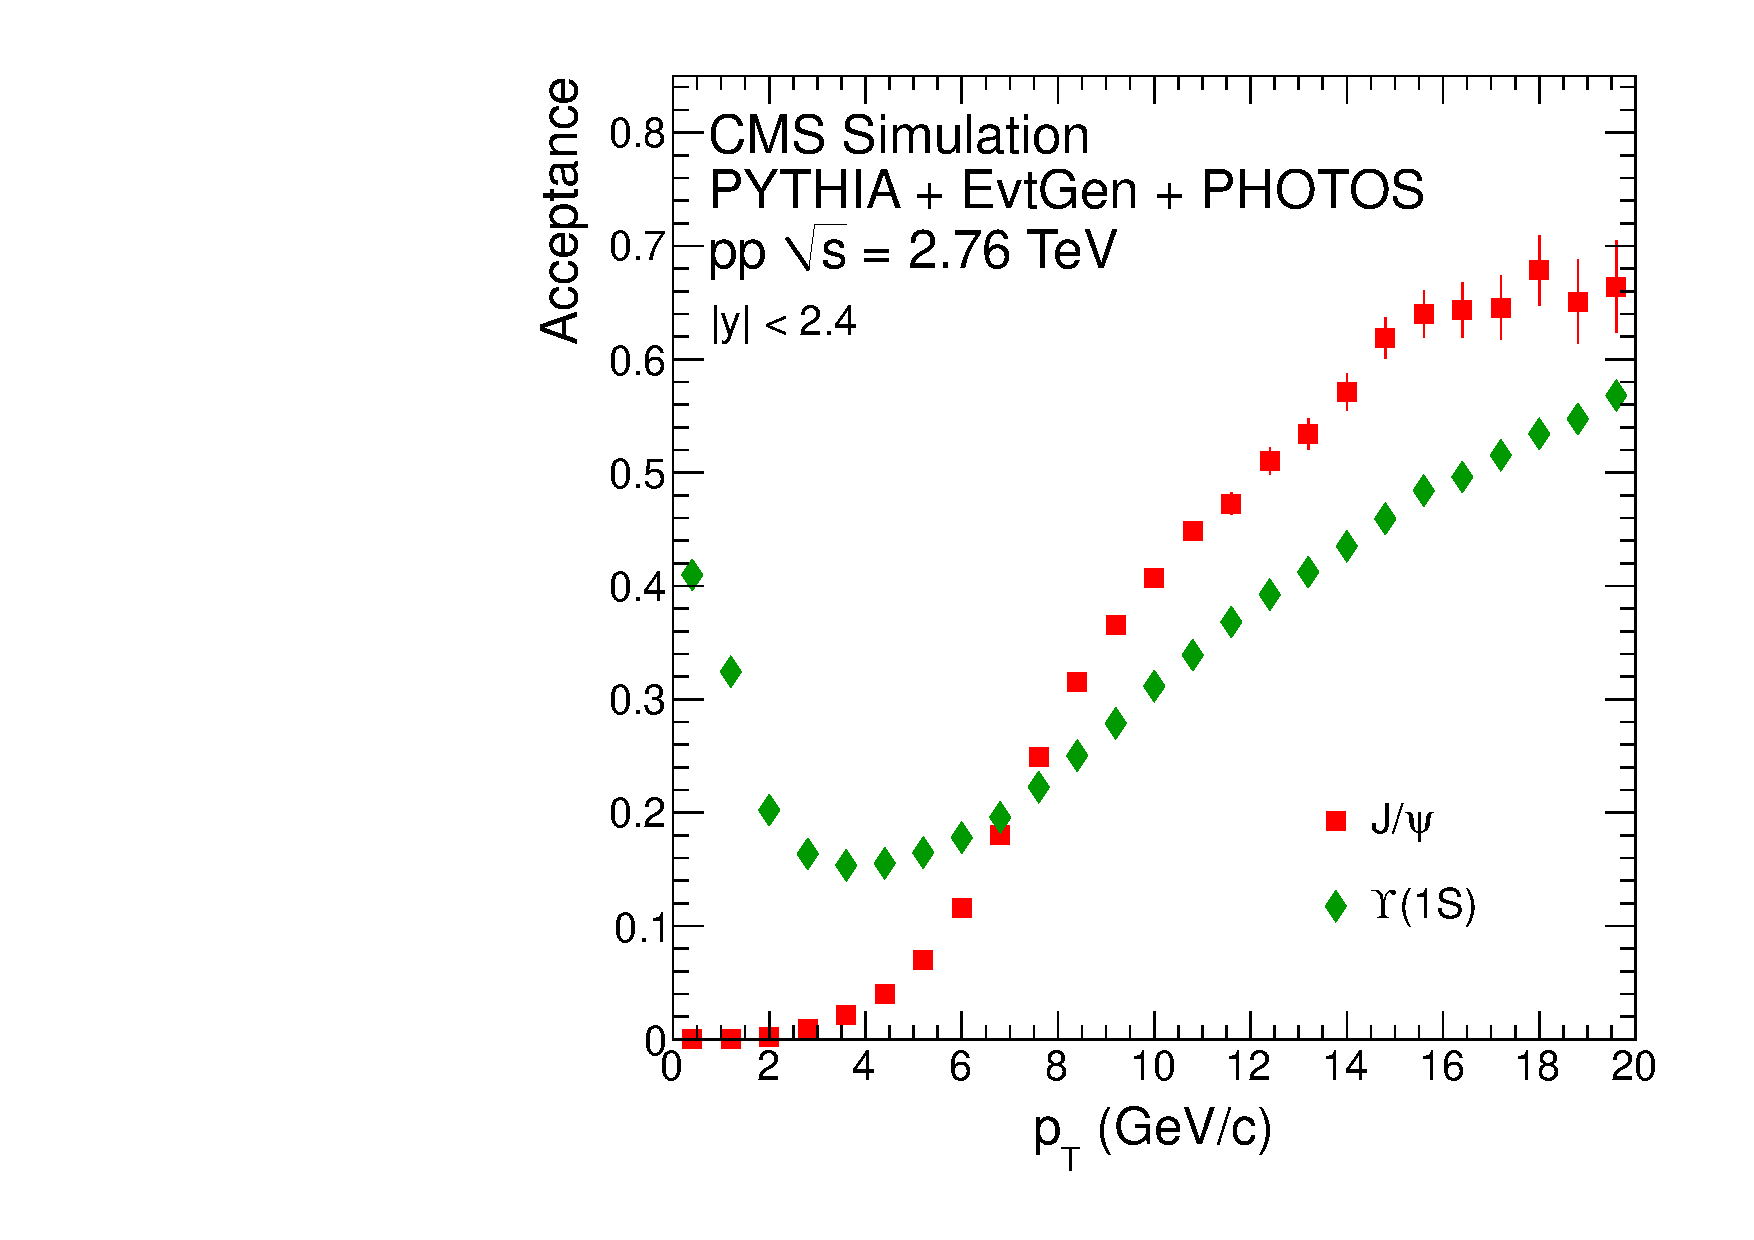
\includegraphics[width=0.45\linewidth]{chap_YInPbPbColl2010_figures/acc_pt_promptJpsi}
  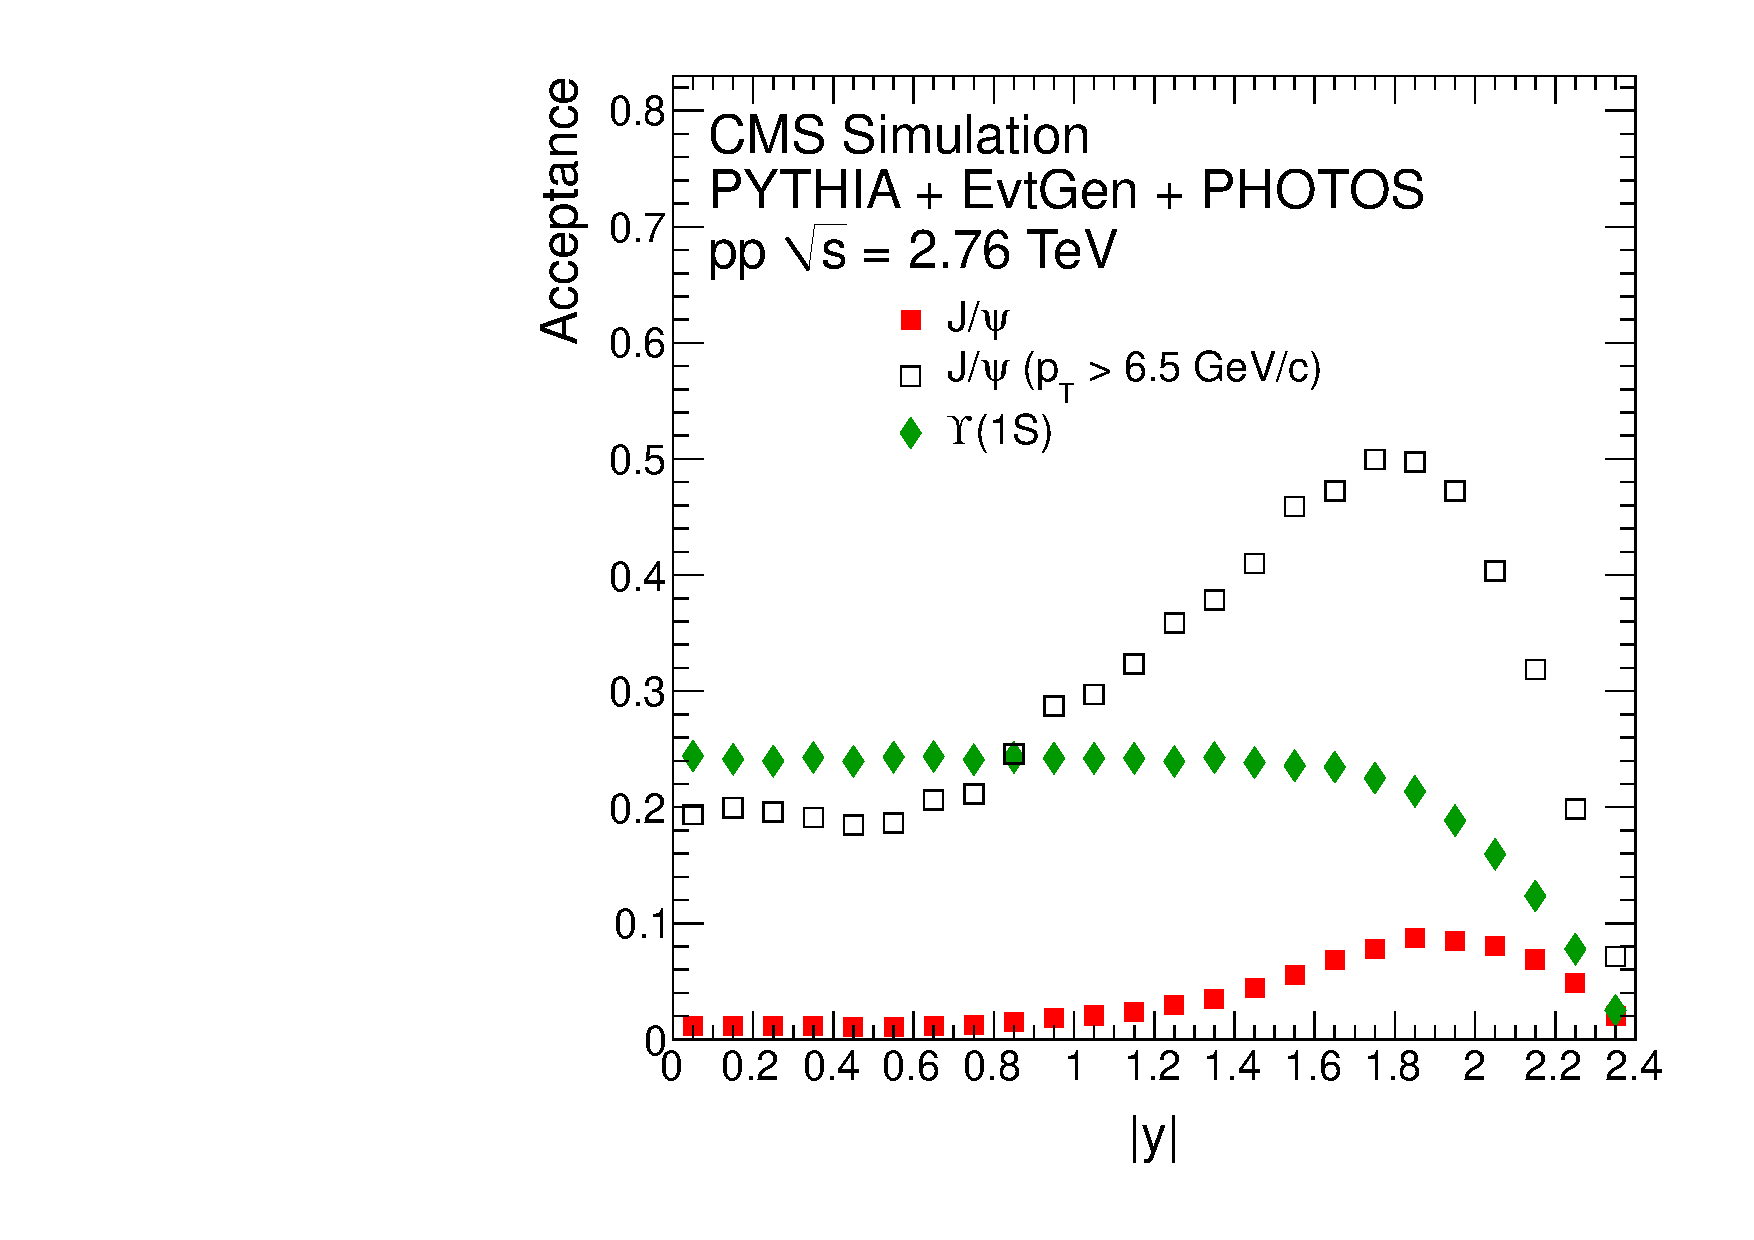
\includegraphics[width=0.45\linewidth]{chap_YInPbPbColl2010_figures/acc_y_promptJpsi}
  \caption{Dimuon acceptance as a function of \pt (left) and $|y|$
    (right) for \Jpsi (red squares) and \PgUa\ (green diamonds). Also
    shown in the right panel is the acceptance for \Jpsi with
    $\pt>6.5\GeVc$ (open black squares). The error bars represent the
    statistical uncertainties only.}
  \label{fig:acceptance}
\end{figure*}
Since the acceptance is a function of both \pt and $y$, uncertainties
in the predicted distributions for these variables can lead to a
systematic uncertainty in the average acceptance over a \pt or $y$
bin.  To estimate these uncertainties, the shapes of the generated MC
\pt and $|y|$ distributions are varied by applying a weight that
increases linearly from 0.7 to 1.3 over the range $0<|y|<2.4$ and
$0<\pt<30\GeVc$ (20\GeVc) for \Jpsi (\PgUa).  The RMS of the resulting
changes in the acceptance for each \pt and $y$ bin are summed in
quadrature to compute the overall systematic uncertainty from this
source.  The largest relative systematic uncertainties obtained are
4.2\%, 3.2\%, and 2.8\% for the prompt \Jpsi, non-prompt \Jpsi, and
\PgUa\ acceptances, respectively.

\subsection{Efficiency}
\label{sec:eff}

The trigger, reconstruction, and selection efficiencies of \mumu pairs
are evaluated using simulated MC signal events embedded in simulated
\PbPb events, as described in Section~\ref{sec:event-sel}. The overall
efficiency is calculated, in each analysis bin, as the fraction of
generated events (passing the single muon phase space cuts) where both
muons are reconstructed, fulfil the quality selection criteria and
pass the trigger requirements. In the embedded sample, the signal over
background ratio is by construction higher than in data, so the
background contribution underneath the resonance peak is negligible
and the signal is extracted by simply counting the \mumu pairs in the
quarkonium mass region. The counting method is crosschecked by using
exactly the same fitting procedure as if the MC events were collision
data. Only muons in the kinematic region defined by
Eqs.~\eqref{eq:singleMuonAcc} and~\eqref{eq:singleMuonAccUps} are
considered.
In \fig{fig:eff}, the efficiencies are shown as a function of the
\mumu pair \pt, $y$, and the event centrality, for each signal: red
squares for prompt \Jpsi, orange stars for non-prompt \Jpsi, and green
diamonds for \PgUa. The efficiency of non-prompt \Jpsi is lower than that 
of prompt \Jpsi, reaching about 35\% for $\pt > 12\GeVc$. 
The prompt \Jpsi efficiency increases with \pt until reaching a plateau 
slightly above 50\% at \pt
of about 12\GeVc, while the \PgUa\ efficiency is $\sim\!55\%$,
independent of \pt. The efficiencies decrease slowly as a function of
centrality because of the increasing occupancy in the silicon tracker;
the relative difference between peripheral and central collisions is
17\% for \Jpsi and 10\% for \PgUa. The integrated efficiency values
are 38.3\%, 29.2\%, and 54.5\% for the prompt \Jpsi, non-prompt \Jpsi
(both with $6.5<\pt<30\GeVc$, $|y|<2.4$, and 0--100\% centrality), and
\PgUa\ (with $0<\pt<20\GeVc$, $|y|<2.4$, and 0--100\% centrality),
respectively.
\begin{figure}[htbp]
  \centering
  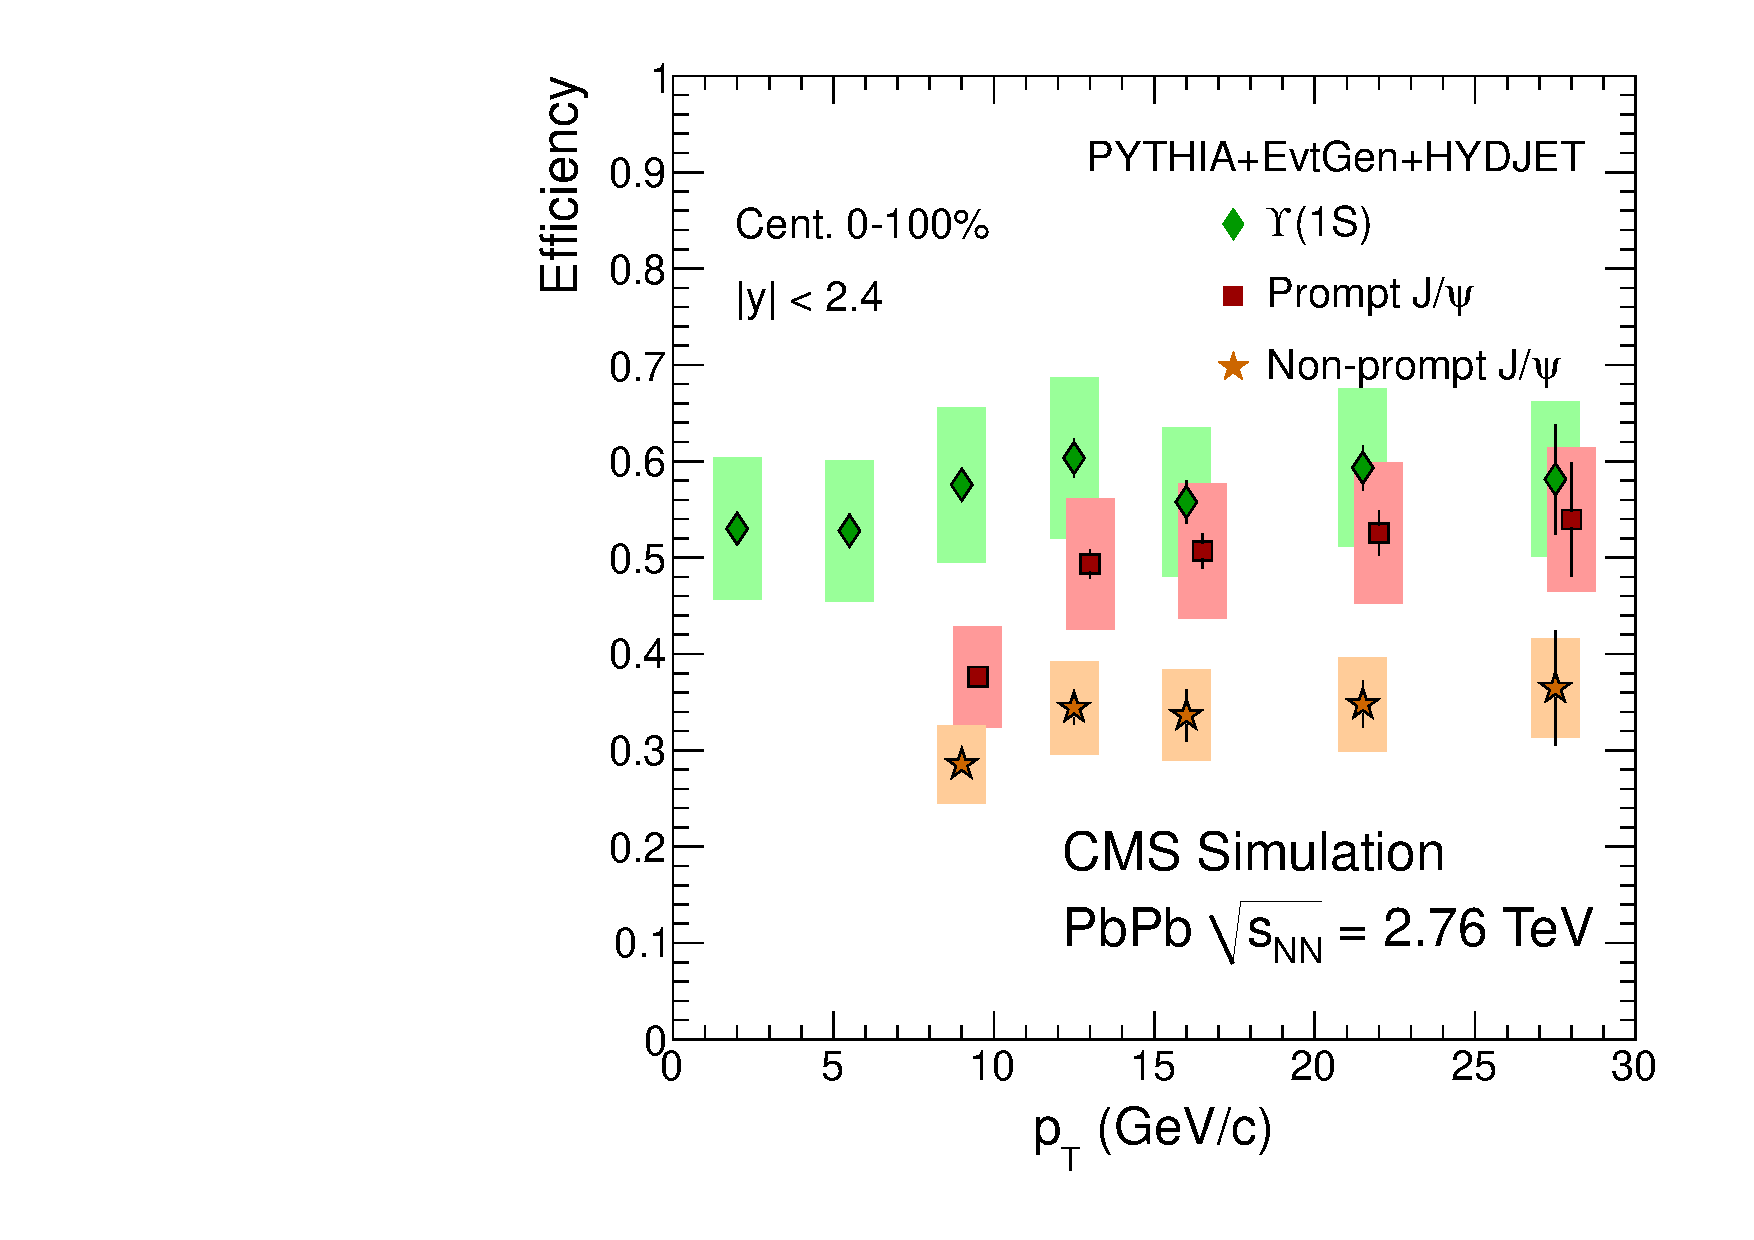
\includegraphics[width=0.45\linewidth]{chap_YInPbPbColl2010_figures/QuarkoniaEff_pt}
  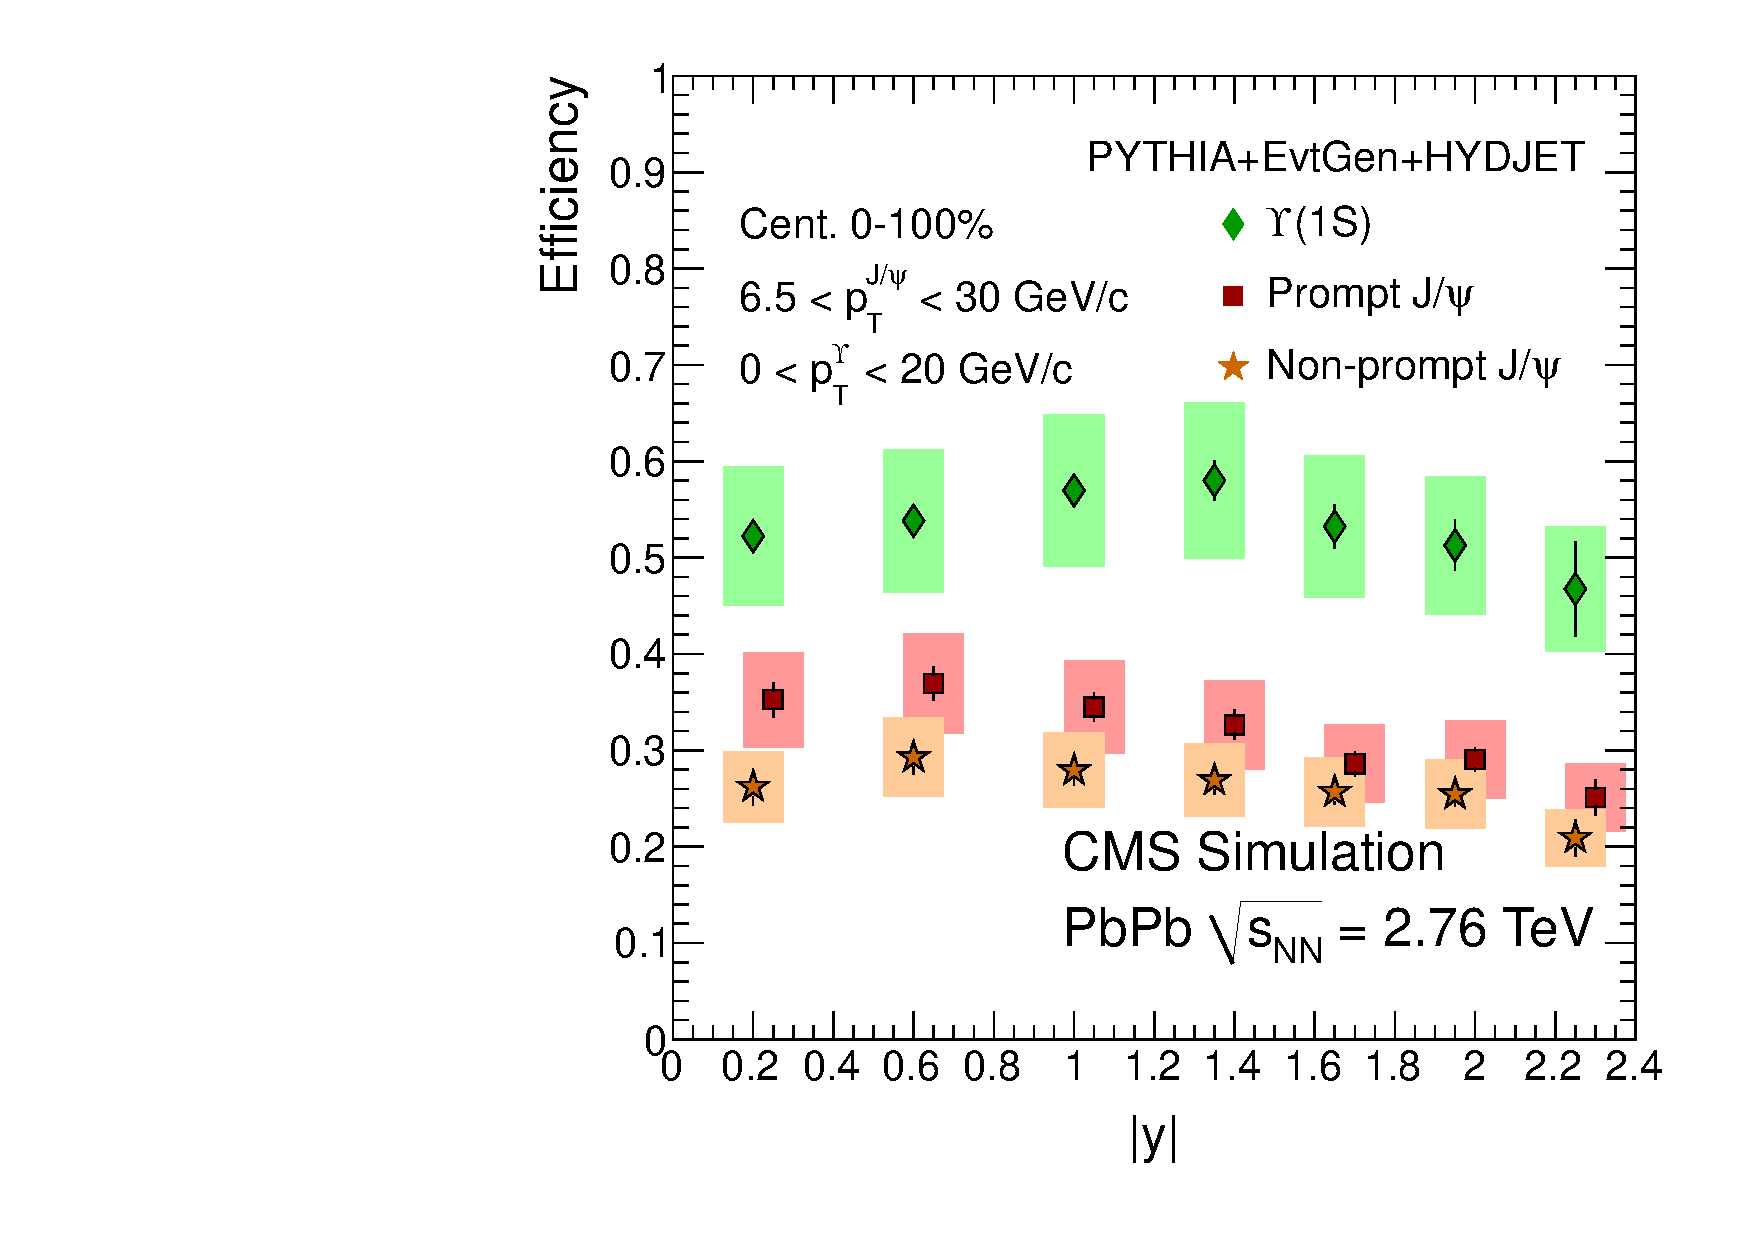
\includegraphics[width=0.45\linewidth]{chap_YInPbPbColl2010_figures/QuarkoniaEff_y}\\
  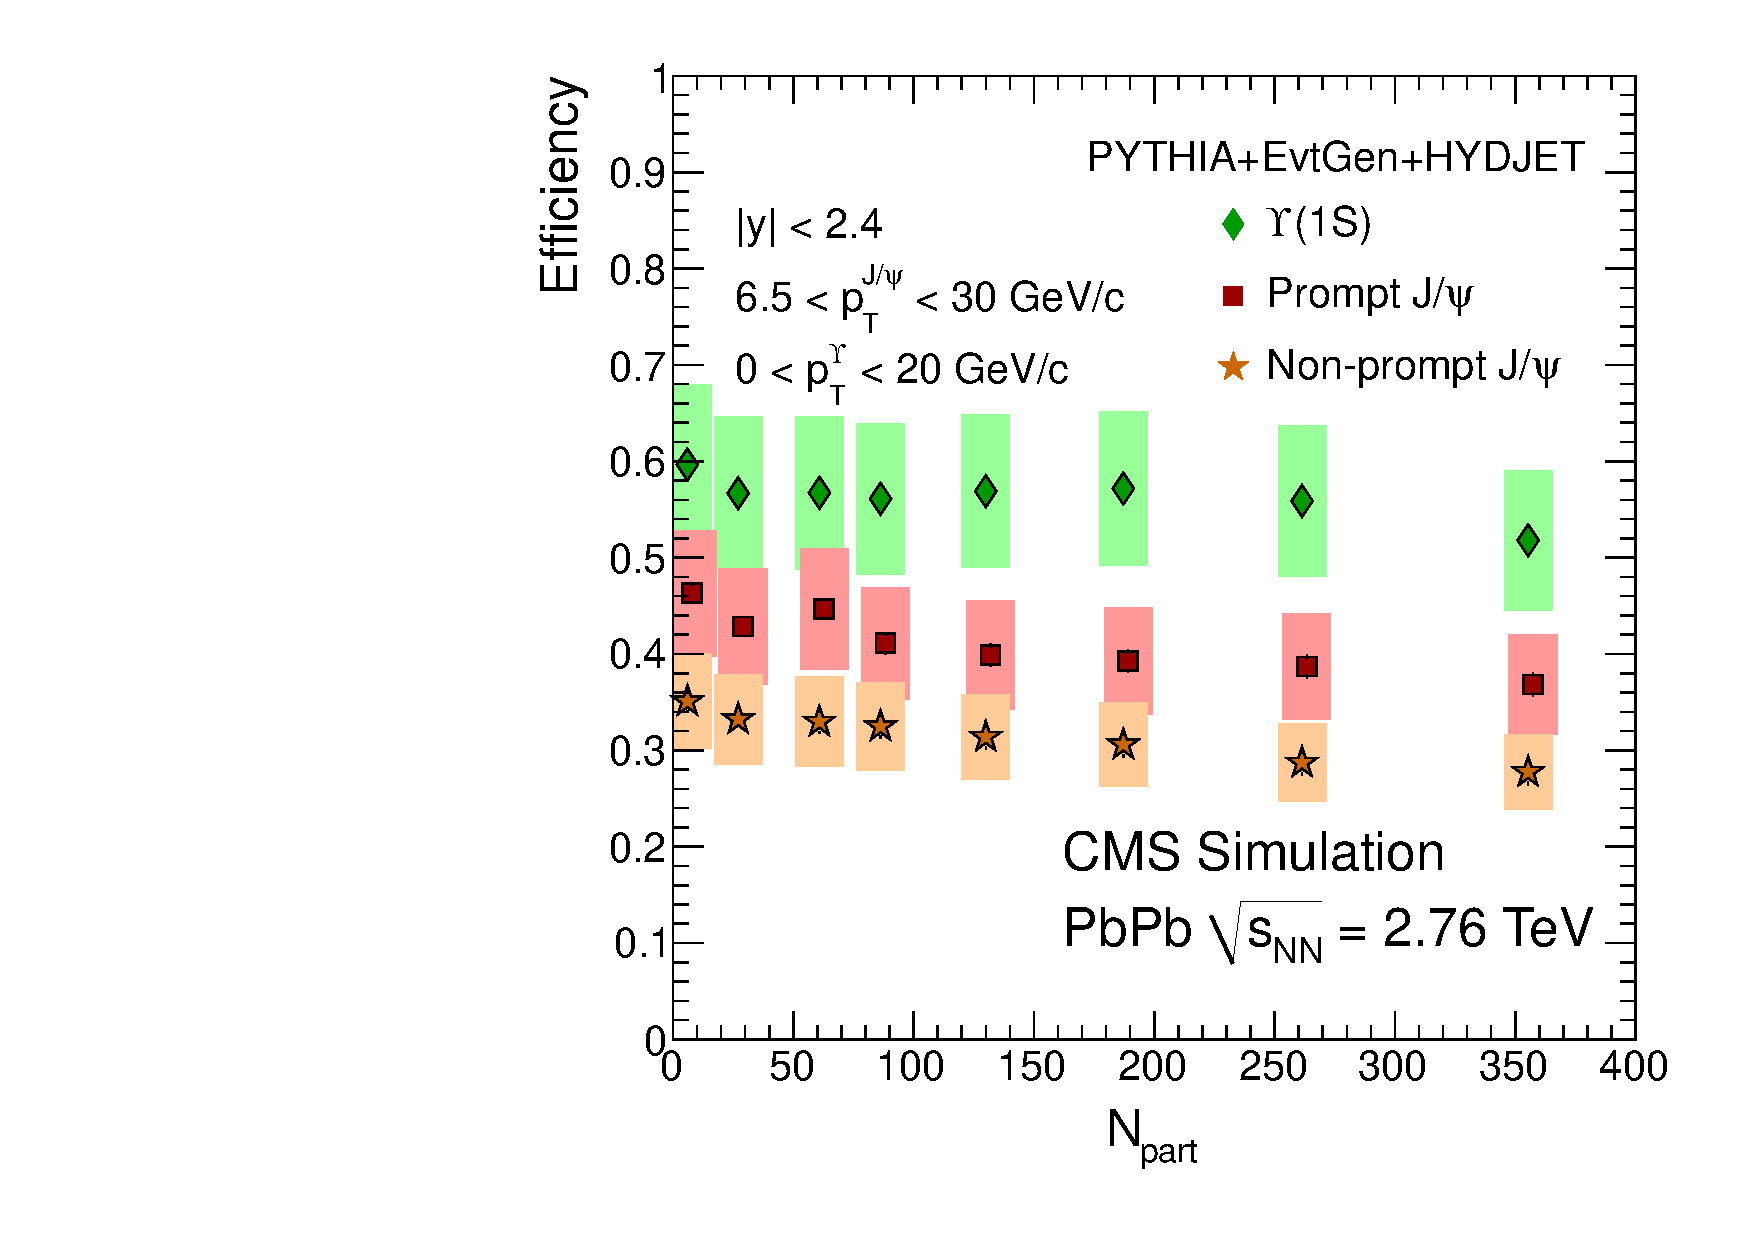
\includegraphics[width=0.45\linewidth]{chap_YInPbPbColl2010_figures/QuarkoniaEff_cent}
  \caption{Combined trigger, reconstruction, and selection
    efficiencies as a function of quarkonium \pt and $|y|$, and event
    centrality, for each signal: red squares and orange stars for
    prompt and non-prompt \Jpsi, respectively, and green diamonds for
    \PgUa. For better visibility, the prompt \Jpsi points are shifted
    by $\Delta \pt = 0.5\GeVc$, $\Delta y=0.05$, and $\Delta \npart =
    2$. Statistical (systematic) uncertainties are shown as bars
    (boxes). The systematic uncertainties are the quadratic sum of the
    uncertainty on the kinematic distributions and the MC validation
    uncertainty.}
  \label{fig:eff}
\end{figure}

The systematic uncertainty on the final corrections due to the
kinematic distributions is estimated by a $\pm30\%$ variation of the
slopes of the generated \pt and rapidity shapes, similar to the
acceptance variation described in the previous section. The systematic
uncertainties are in the ranges 1.8--3.4\%, 2.2--4.2\%, and 1.4--2.7\%
for prompt \Jpsi, non-prompt \Jpsi, and \PgUa, respectively, including
the statistical precision of the MC samples.
The individual components of the MC efficiency are crosschecked using
muons from \Jpsi decays in simulated and collision data with a
technique called \emph{tag-and-probe}, similar to the one used for the
corresponding \pp measurement~\cite{Khachatryan:2010yr}.

\section{The pp Baseline Measurement}
\label{sec:ppRef}
A \pp run at \sqrts = 2.76\TeV was taken in March 2011. The integrated
luminosity was 231 nb$^{-1}$, with an associated uncertainty of 6\%. For
hard-scattering processes, the integrated luminosity of the \pp sample
is comparable to that of the \PbPb sample (\mbox{$7.28 \mu\,b^{-1} \cdot
208^2 \approx 315 nb^{-1}$}).

Given the higher instantaneous luminosity, the 
trigger required
slightly higher quality muons in the \pp run than in the \PbPb
run. The offline event selection is the same as in the \PbPb analysis,
only slightly relaxed for the HF coincidence requirement: instead of
three towers, only one tower with at least 3 GeV deposited is required
in the \pp case. The same reconstruction algorithm, i.e. the one
optimized for the heavy-ion environment, is used for both \pp and
\PbPb data. The products of the trigger, reconstruction, and selection
efficiencies determined in \pp MC simulations are 42.5\%, 34.5\%, and
55.1\% for the prompt \Jpsi, non-prompt \Jpsi (both with
$6.5<\pt<30\GeVc$, $|y|<2.4$), and \PgUa\ (with $0<\pt<20\GeVc$,
$|y|<2.4$), respectively.
The quarkonium signals in \pp collisions are extracted following the
same methods as in \PbPb collisions.

The invariant-mass spectrum of \mumu pairs in the $\PgU$ region from
\pp collisions is shown in \fig{fig:ups_pp}. The same procedure as the
one described for the \PbPb analysis is used. The number of $\PgUa$
mesons with $|y|<2.4$ and $0<\pt<20\,\GeV/c$ is $101\pm12$. The fit
result of the excited states is discussed in~\cite{Chatrchyan:2011pe}.

\begin{figure}[hbtp]
  \begin{center}
  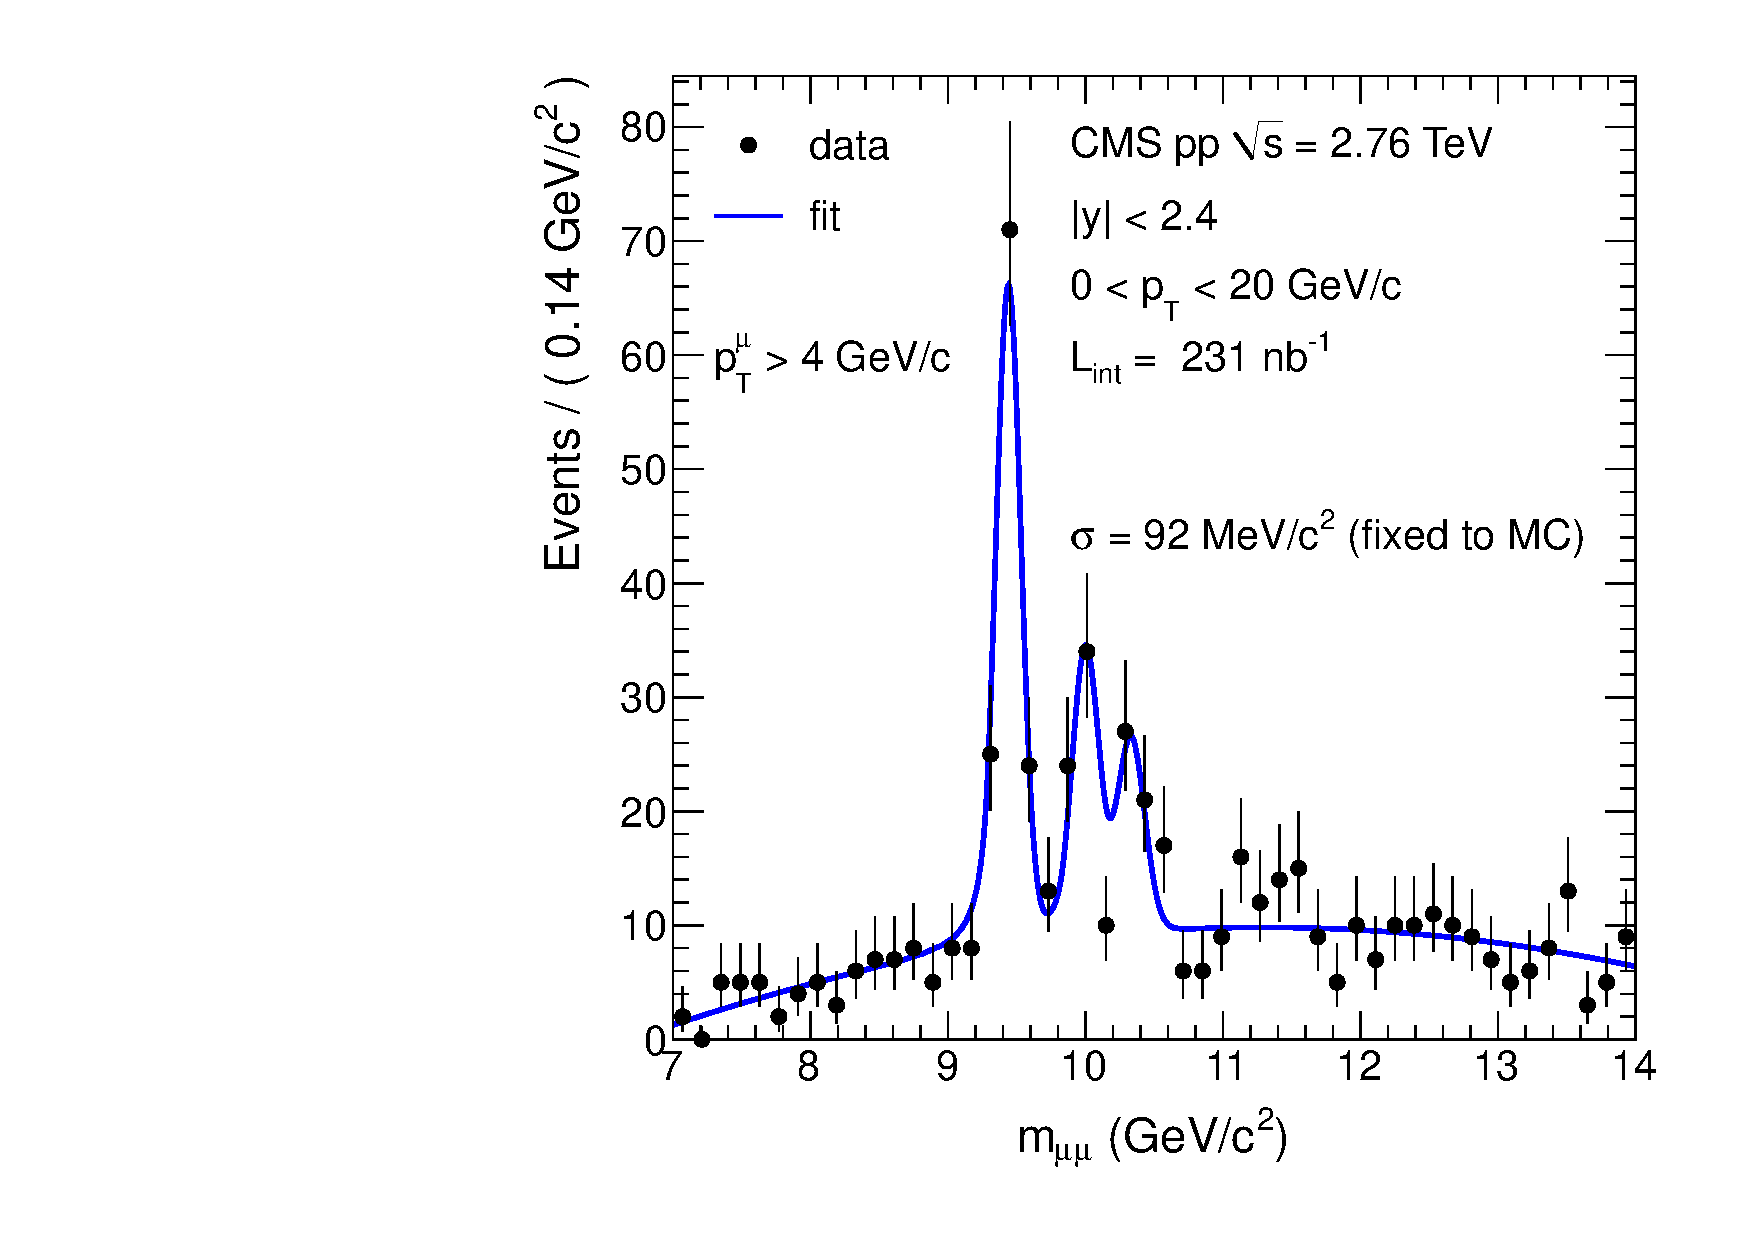
\includegraphics[width=0.5\linewidth]{chap_YInPbPbColl2010_figures/masspeak_pp_HIrereco}
  \caption{The \pp dimuon invariant-mass distribution in the range
    $\pt<20 \GeVc$ for $|y|<2.4$ and the result of the fit to the
    $\PgU$ resonances.}
  \label{fig:ups_pp}
  \end{center}
\end{figure}

For the measurement of the nuclear modification factors, in which the
ratio of \PbPb to \pp results is computed, most of the reconstruction
systematic uncertainties cancel out because the same algorithm is
used. However, the following factors must be accounted for:

\begin{enumerate}
\item The luminosity uncertainty. This is a global systematic
  uncertainty of 6\% that allows all measured nuclear modification
  factors to change by a common scale-factor. Since the \PbPb yield is
  normalized by the number of minimum-bias events, which has a
  negligible uncertainty, no systematic uncertainty on the \PbPb
  luminosity has to be considered.
\item The uncertainty on \taa. For results integrated over centrality,
  this is a global systematic uncertainty of 5.7\%, based on the
  Glauber model employed. For results as a function of centrality, the
  uncertainty varies between a minimum of 4.3\% in the most central
  bin and a maximum of 15\% in the most peripheral
  bin~\cite{Chatrchyan:2011sx}.
\item The systematic uncertainty associated with the trigger
  efficiency. The ratios between the \emph{tag-and-probe} efficiencies
  obtained in \pp and \PbPb are the same in data and MC events, within
  the statistical accuracy of the data (1\% for the single-muon
  efficiency).  Twice this value (2\%) is assigned as the uncertainty
  on the difference of the trigger efficiencies of \mumu pairs in
  \PbPb and \pp collisions.
\item The tracking efficiency uncertainty due to different charged
  particle multiplicities in \pp and \PbPb collisions.  The ratios
  between the \emph{tag-and-probe} efficiencies obtained in \pp and
  central \PbPb events are the same in data and MC events, within the
  statistical accuracy of the data (6.8\% for the single-muon
  efficiency).  This value is propagated as the tracking systematic
  uncertainty in all the ratios of \PbPb to \pp data.
\end{enumerate}

\section{Results}
\label{sec:results}

The double-differential quarkonium cross sections in \PbPb collisions
are reported in the form
\begin{equation}
  \label{eq:xsection}
    \frac{1}{\taa} \cdot
    \frac{\mathrm{d}^2N}{\mathrm{d}y\,\mathrm{d}\pt} = \frac{1}{\taa\, N_{\text{MB}}} \cdot \frac{1}{\Delta y\, \Delta \pt} \cdot \frac{N_{\QQbar}}{A\, \varepsilon},
\end{equation}
while in \pp collisions they are calculated as
\begin{equation}
  \label{eq:xsection_pp}
    \frac{d^2\sigma}{\mathrm{d}y\,\mathrm{d}\pt} = \frac{1}{L_{\pp}} \cdot \frac{1}{\Delta y\, \Delta \pt} \cdot \frac{N_{\QQbar}}{A\, \varepsilon},
\end{equation}
where:
\begin{itemize}
\item $N_{\QQbar}$ is the number of measured \PgUa\ in the \mumu decay channel;
\item $N_{\text{MB}}$ is the number of minimum-bias events sampled by
  the event selection; when binned in centrality, only the fraction of
  minimum-bias events in that centrality bin is considered;
\item $A$ is the geometric acceptance, which depends on the \pt and $y$
  of the quarkonium state;
\item $\varepsilon$ is the combined trigger and reconstruction
  efficiency, which depends on the \pt and $y$ of the quarkonium state
  and on the centrality of the collision;
\item $\Delta y$ and $\Delta \pt$ are the bin widths in rapidity and
  \pt, respectively;
\item \taa is the nuclear overlap function, which depends on the
  collision centrality;
\item $L_{\pp} = (231\pm14) \rm nb^{-1}$ is the integrated luminosity of
  the \pp data set.
\end{itemize}

Following \eq{eq:xsection}, the uncorrected yields of \PgUa, measured in \PbPb collisions
are corrected for acceptance and efficiency (reported in
Figs.~\ref{fig:acceptance} and \ref{fig:eff}), and converted into
yields divided by the nuclear overlap function \taa. These quantities
can be directly compared to cross sections in \pp collisions measured
from the raw yields according to \eq{eq:xsection_pp}. The rapidity and
centrality-dependent results are presented integrated over \pt. All
results are presented for the unpolarized scenario and are tabulated
in Tables~\ref{tab:inclxsec}--\ref{tab:upsilonxsectpp} of
Appendix~\ref{app:datatables}.

The systematic uncertainties detailed in the previous sections are
summarized in Tables~\ref{tab:syst_PbPb} and~\ref{tab:syst_pp}. The
relative uncertainties for all terms appearing in
Eqs.~(\ref{eq:xsection}) and~(\ref{eq:xsection_pp}) are added in
quadrature, leading to a total of 15--21\% on the corrected
yields. For results plotted as a function of \pt or rapidity, the
systematic uncertainty on \taa enters as a global uncertainty on the
scale and is not included in the systematic uncertainties of the
yields. As a function of centrality, the uncertainty on \taa varies
point-to-point and is included in the systematic uncertainties of the
yields.

\begin{table}[htbp]
  \begin{center}
    \caption{Point-to-point systematic uncertainties on
      the prompt \Jpsi, non-prompt \Jpsi, and \PgUa\ yields measured in
      \PbPb collisions.}
    \label{tab:syst_PbPb}
    \begin{tabular}{lr@{--}lr@{--}lr@{--}l}
      \hline
      ~ & \multicolumn{2}{c}{prompt \Jpsi (\%)} & \multicolumn{2}{c}{non-prompt \Jpsi (\%)} & \multicolumn{2}{c}{\PgUa\ (\%)}\\\hline
      Yield extraction & 0.5&5.7 & 1.5&14.0 & 8.7&13.4\\
      Efficiency & 1.8&3.4 & 2.2&4.2 & 1.4&2.7\\
      Acceptance & 0.9&4.2 & 2.0&3.2 & 1.5&2.8\\
      MC Validation & \multicolumn{2}{l}{13.7} & \multicolumn{2}{l}{13.7} & \multicolumn{2}{l}{13.7}\\
      Stand-alone $\mu$ reco. & \multicolumn{2}{l}{1.0} & \multicolumn{2}{l}{1.0} & \multicolumn{2}{l}{1.0}\\
      \taa & 4.3&15.0 & 4.6&8.6 & 4.3&8.6\\\hline
      Total & 15&21 & 15&21 & 18&20\\\hline
    \end{tabular}
  \end{center}
\end{table}

\begin{table}[htbp]
  \begin{center}
    \caption{Point-to-point systematic uncertainties on
      the prompt \Jpsi, non-prompt \Jpsi, and \PgUa\ yields measured in
      \pp collisions.}
    \label{tab:syst_pp}
    \begin{tabular}{lr@{--}lr@{--}lr@{--}l}
      \hline
      ~ & \multicolumn{2}{c}{prompt \Jpsi (\%)} & \multicolumn{2}{c}{non-prompt \Jpsi (\%)} & \multicolumn{2}{c}{\PgUa\ (\%)}\\\hline
      Yield extraction & 0.8&5.3 & 5.3&16.8 & \multicolumn{2}{l}{10.0}\\
      Efficiency & 1.6&3.0 & 1.4&2.0 & 0.4&0.9\\
      Acceptance & 0.9&4.2 & 2.0&3.2 & 1.5&2.8\\
      MC Validation & \multicolumn{2}{l}{13.7} & \multicolumn{2}{l}{13.7} & \multicolumn{2}{l}{13.7}\\
      Stand-alone $\mu$ reco. & \multicolumn{2}{l}{1.0} & \multicolumn{2}{l}{1.0} & \multicolumn{2}{l}{1.0}\\\hline
      Total & 14&16 & 15&22 & 17&18\\\hline
    \end{tabular}
  \end{center}
\end{table}
The nuclear modification factor,
\begin{equation}
    \raa = \frac{L_{\pp}}{\taa N_{\text{MB}}}\frac{N_{\PbPb} (\QQbar)}{N_{\pp} (\QQbar)}\cdot \frac{\varepsilon_{\pp}}{\varepsilon_{\PbPb}}\,,
\end{equation}
is calculated from the raw yields $N_{\PbPb} (\QQbar)$ and $N_{\pp}
(\QQbar)$, correcting only for the multiplicity-dependent fraction of
the efficiency ($\frac{\varepsilon_{\pp}}{\varepsilon_{\PbPb}}
\sim\!1.16$ for the most central bin); the \pt and rapidity
dependencies of the efficiency cancel in the ratio. These results are
also tabulated in Appendix~\ref{app:datatables}. It should be noted
that the \raa would be sensitive to changes of the \Jpsi polarization
between \pp and \PbPb collisions, an interesting physics effect on its
own~\cite{Faccioli:2012kp}.

In all figures showing results, statistical uncertainties are
represented by error bars and systematic uncertainties by
boxes. Results as a function of rapidity are averaged over the
positive and negative rapidity regions.

\subsection{\texorpdfstring{\PgUa}{Upsilon(1S)}}
\label{sec:upsResults}

In \fig{fig:upsilon_pt}, the \PgUa\ yield divided by \taa in \PbPb
collisions and its cross section in \pp collisions are shown as a
function of \pt; the \raa of \PgUa\ is displayed in the right panel of
\fig{fig:upsilon_pt}. The \pt dependence shows a significant
suppression, by a factor of $\sim\!2.3$ at low \pt, that disappears
for $\pt > 6.5\GeVc$. The rapidity dependence indicates a slightly
smaller suppression at forward rapidity, as shown in
\fig{fig:upsilon_eta}. However, the statistical uncertainties are too
large to draw strong conclusions on any \pt or rapidity
dependence. The \PgUa\ yield in \PbPb collisions divided by \taa and
the \PgUa\ \raa are presented as a function of \npart in the left and
right panels of \fig{fig:upsilon_cent}, respectively. Within
uncertainties, no centrality dependence of the \PgUa\ suppression is
observed.

\begin{figure}[htbp]
  \begin{center}
    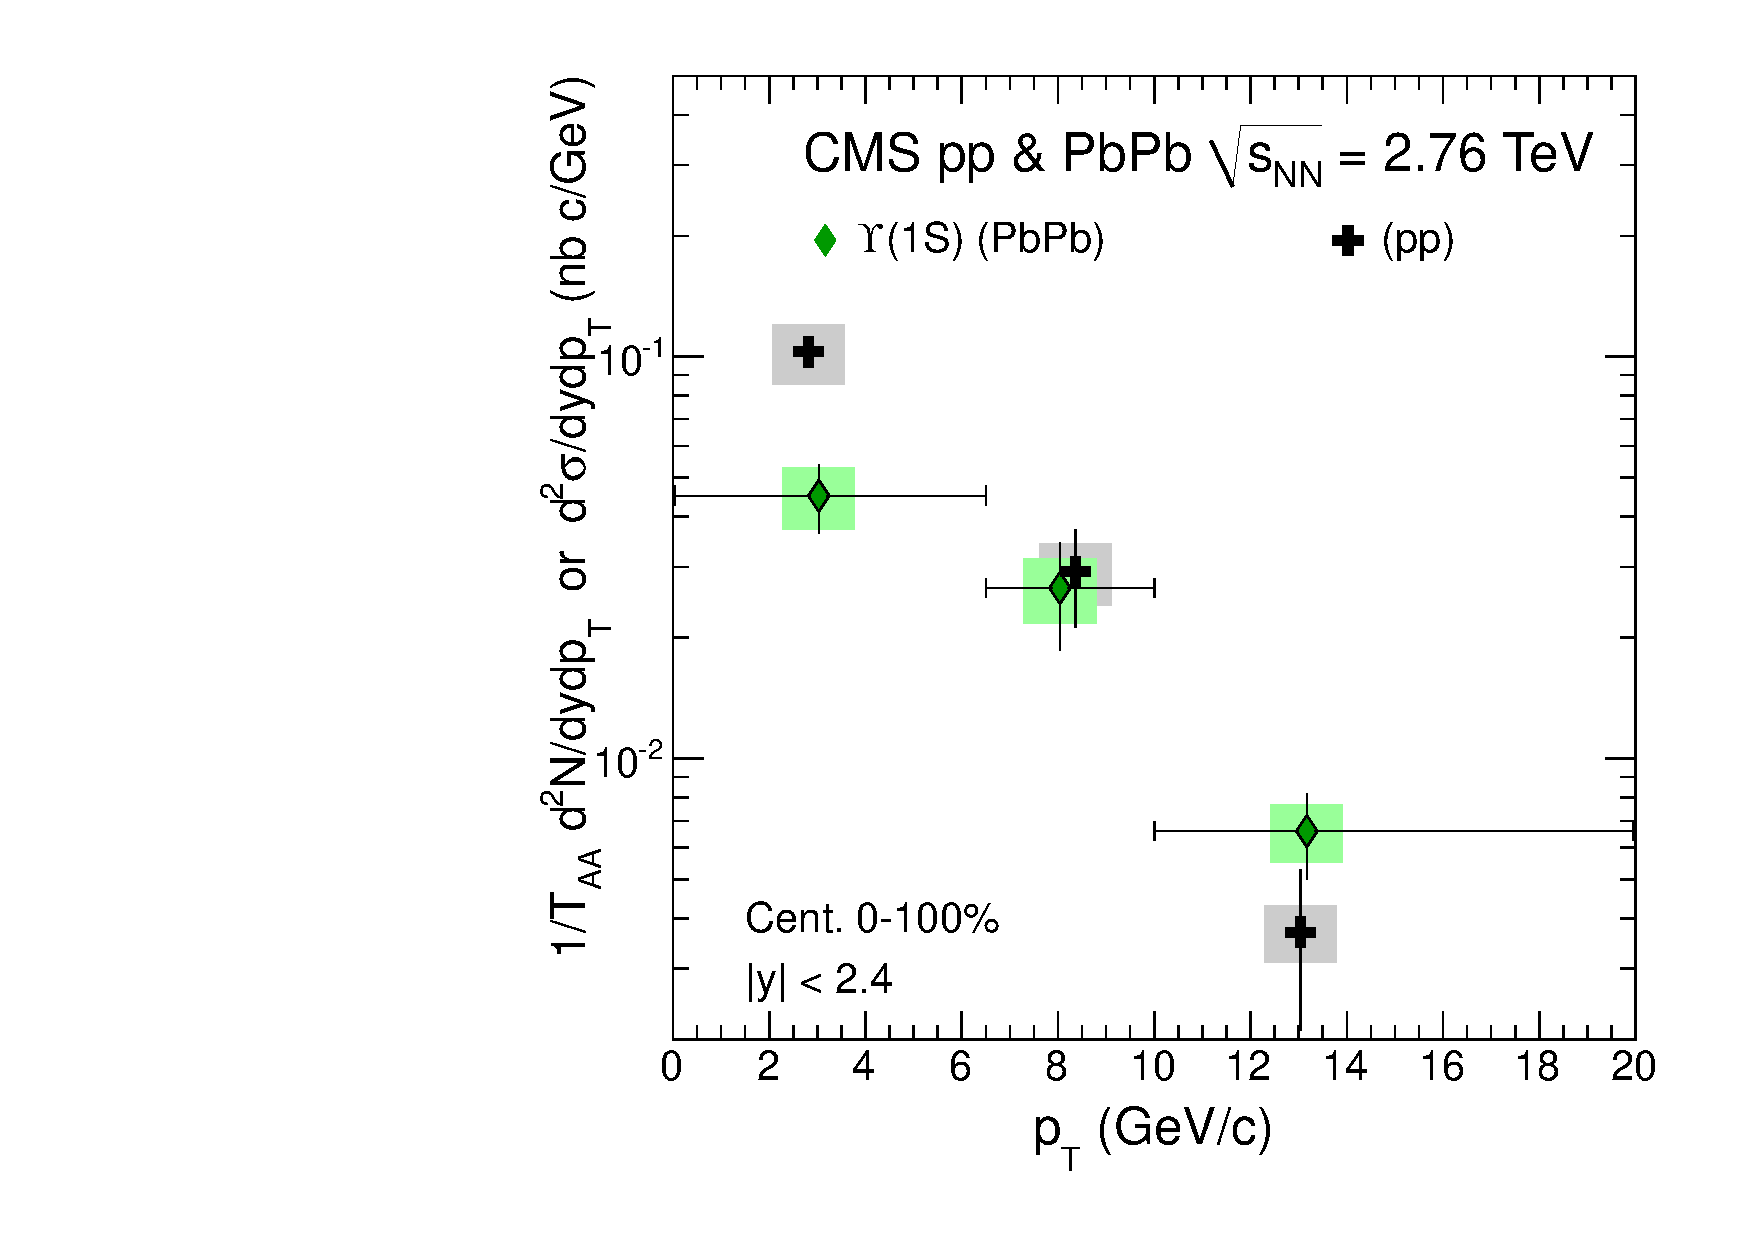
\includegraphics[width=0.45\textwidth]{chap_YInPbPbColl2010_figures/upsilon_pt}\hspace{1em}
    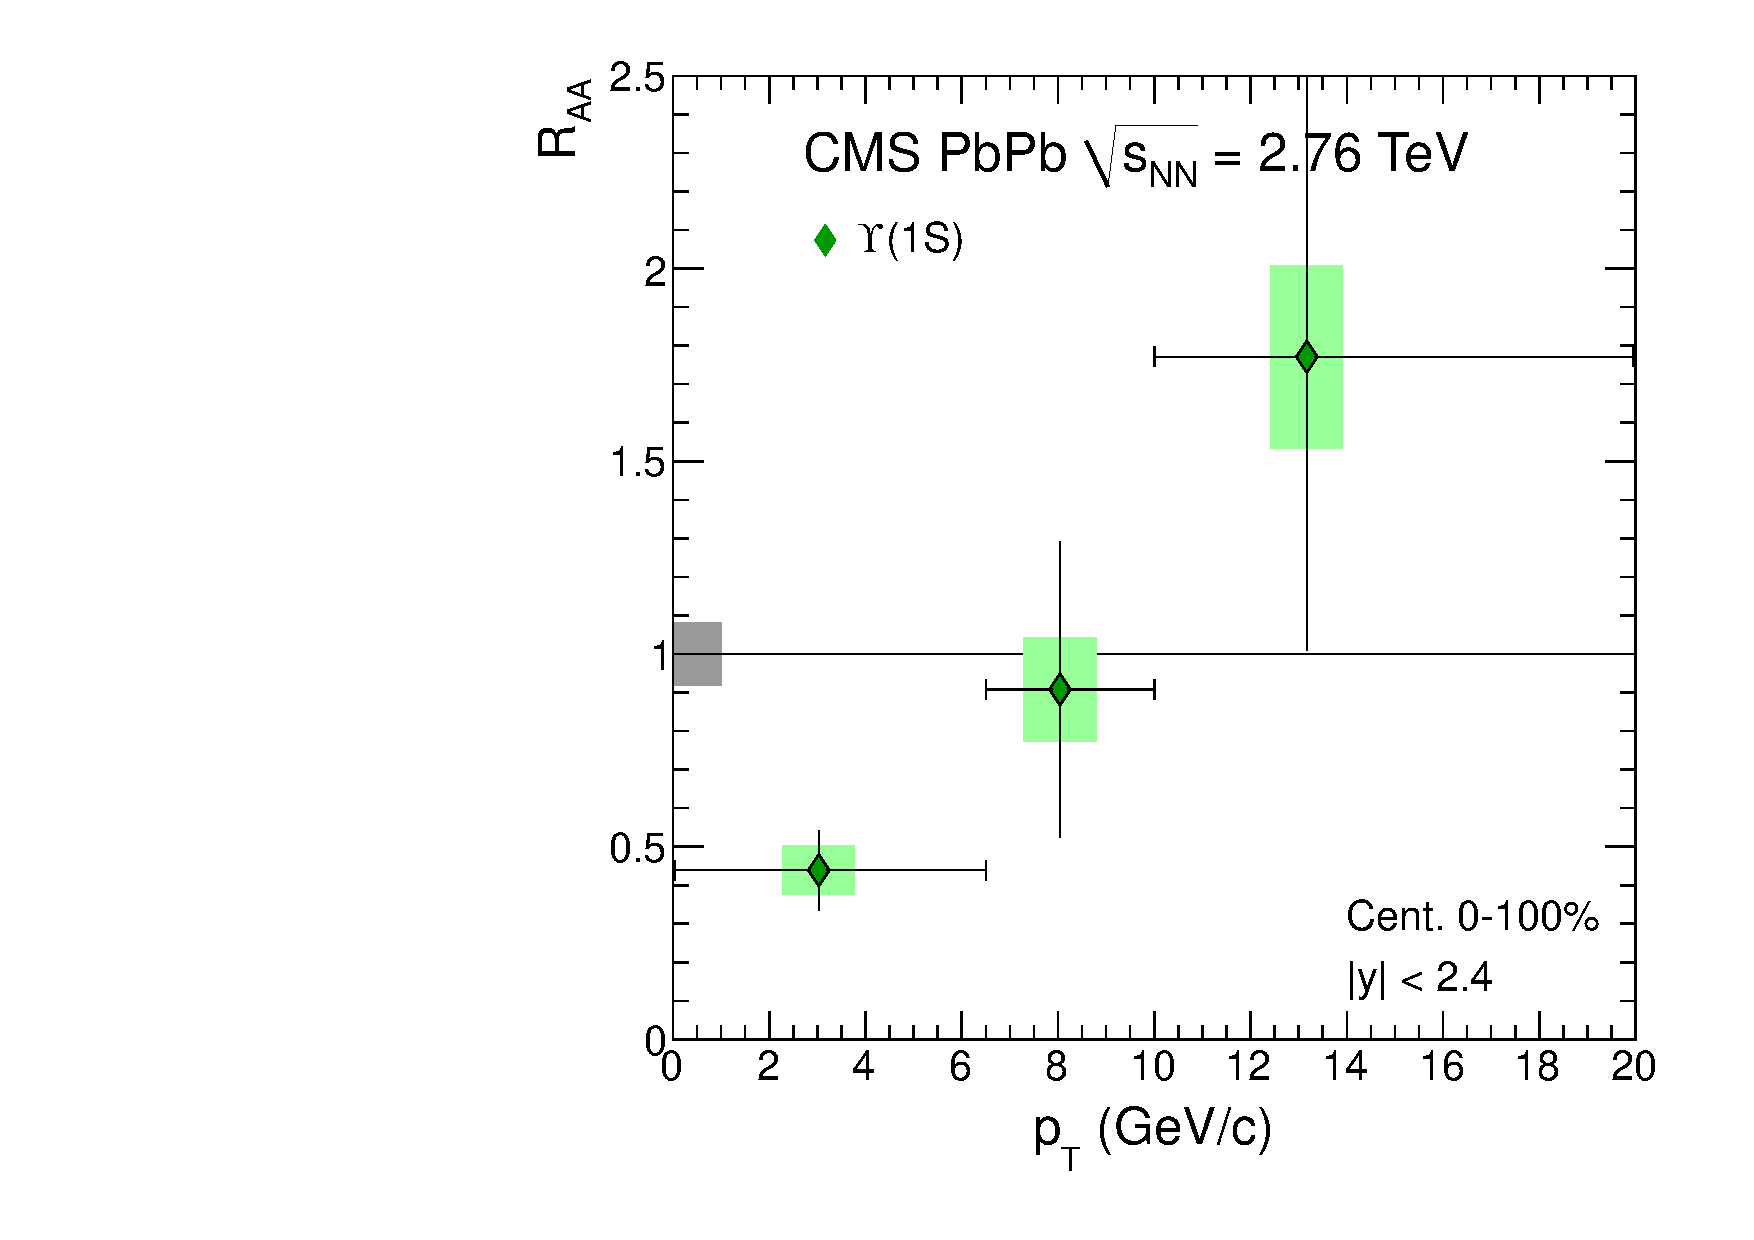
\includegraphics[width=0.45\textwidth]{chap_YInPbPbColl2010_figures/upsilon_RAA_pt}
    \caption{Left: \PgUa\ yield divided by \taa in \PbPb collisions
      (green diamonds) as a function of \pt. The result is compared to
      the cross section measured in \pp collisions (black crosses).
      The global scale uncertainties on the \PbPb data due to \taa
      (5.7\%) and the \pp integrated luminosity (6.0\%) are not
      shown. Right: nuclear modification factor \raa of \PgUa\ as a
      function of \pt. A global uncertainty of 8.3\%, from \taa and
      the integrated luminosity of the \pp data sample, is shown as a
      grey box at $\raa=1$. Points are plotted at their measured
      average \pt. Statistical (systematic) uncertainties are shown as
      bars (boxes). Horizontal bars indicate the bin width.}
    \label{fig:upsilon_pt}
  \end{center}
\end{figure}

\begin{figure}[htbp]
  \begin{center}
    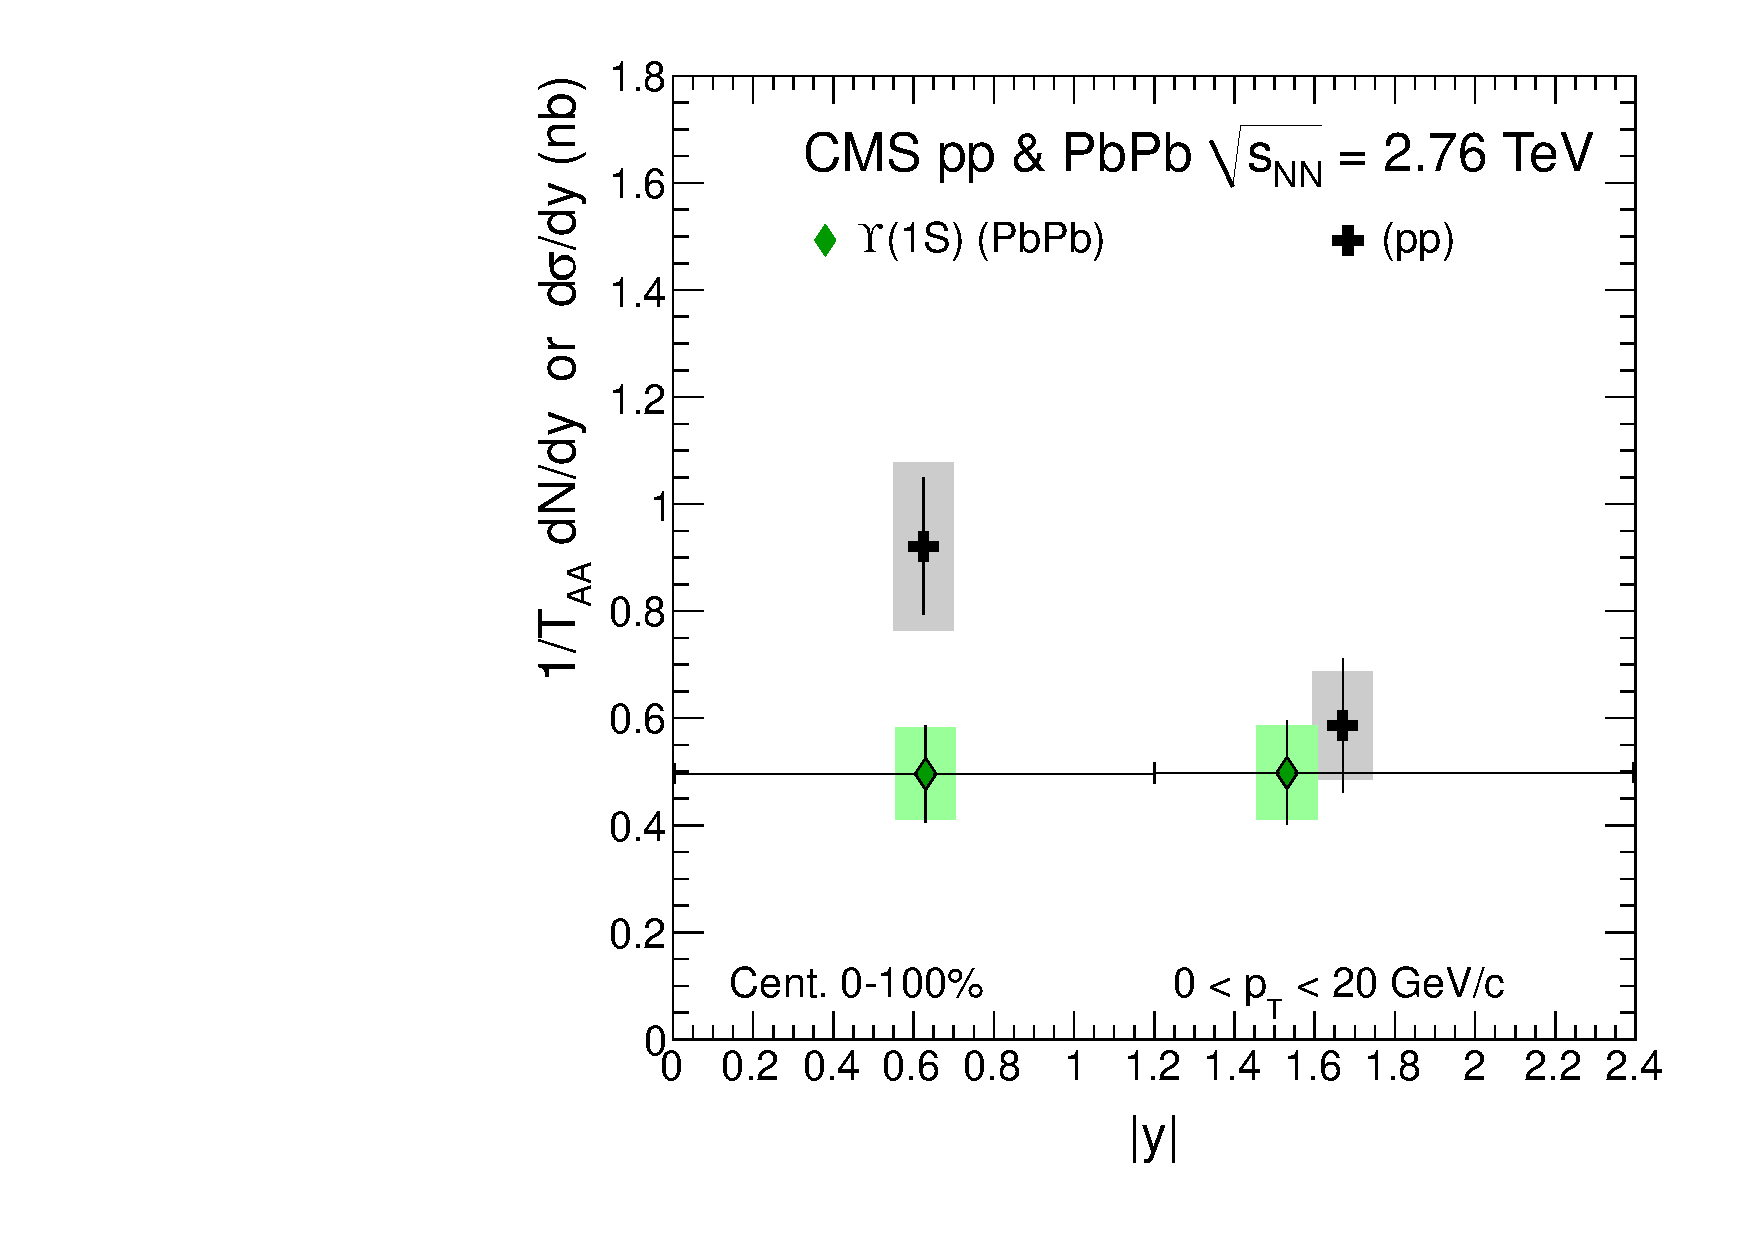
\includegraphics[width=0.45\textwidth]{chap_YInPbPbColl2010_figures/upsilon_eta}\hspace{1em}
    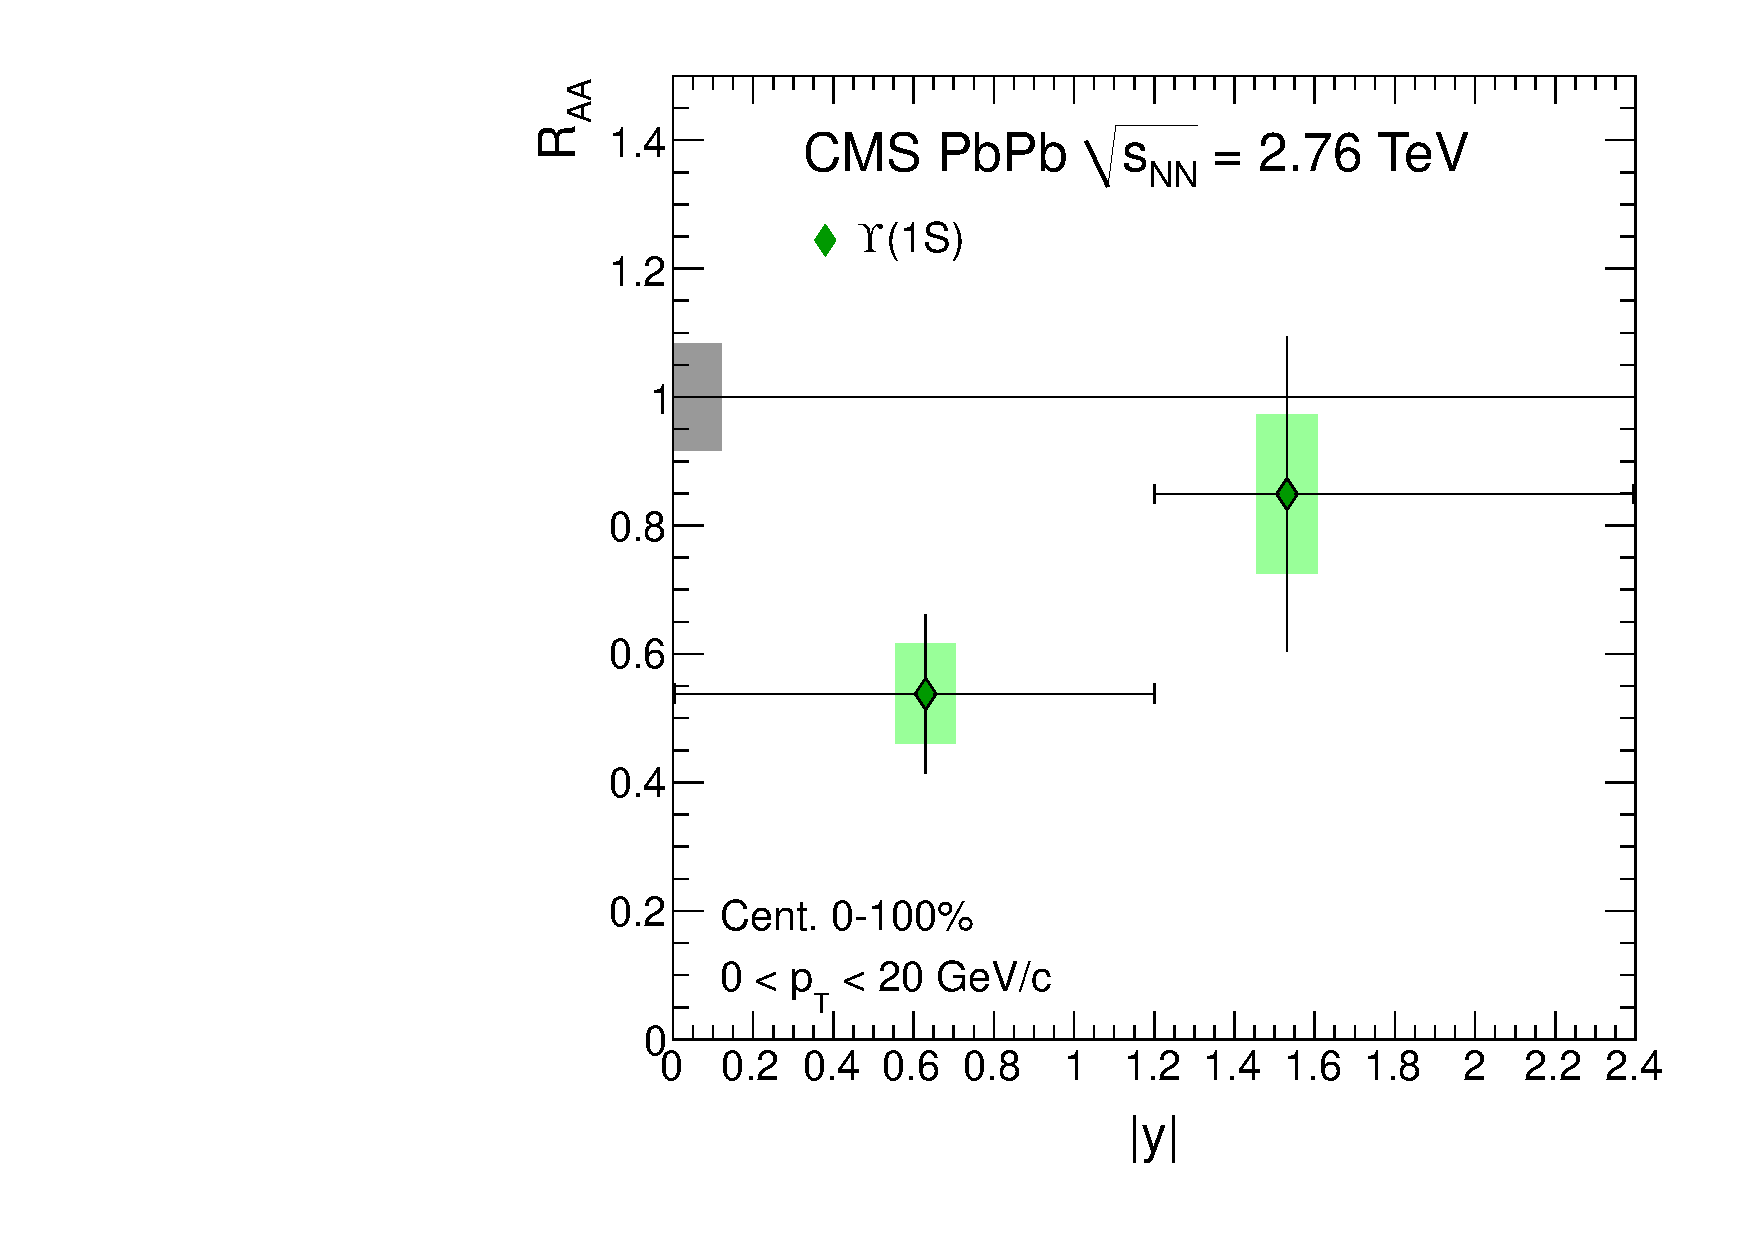
\includegraphics[width=0.45\textwidth]{chap_YInPbPbColl2010_figures/upsilon_RAA_eta}
    \caption{Left: \PgUa\ yield divided by \taa in \PbPb collisions
      (green diamonds) as a function of rapidity. The result is
      compared to the cross section measured in \pp collisions (black
      crosses). The global scale uncertainties on the \PbPb data due
      to \taa (5.7\%) and the \pp integrated luminosity (6.0\%) are
      not shown. Right: nuclear modification factor \raa of \PgUa\ as a
      function of rapidity. A global uncertainty of 8.3\%, from \taa
      and the integrated luminosity of the \pp data sample, is shown
      as a grey box at $\raa=1$. Points are plotted at their measured
      average $|y|$. Statistical (systematic) uncertainties are shown
      as bars (boxes). Horizontal bars indicate the bin width.}
    \label{fig:upsilon_eta}
  \end{center}
\end{figure}
\begin{figure}[htbp]
  \begin{center}
    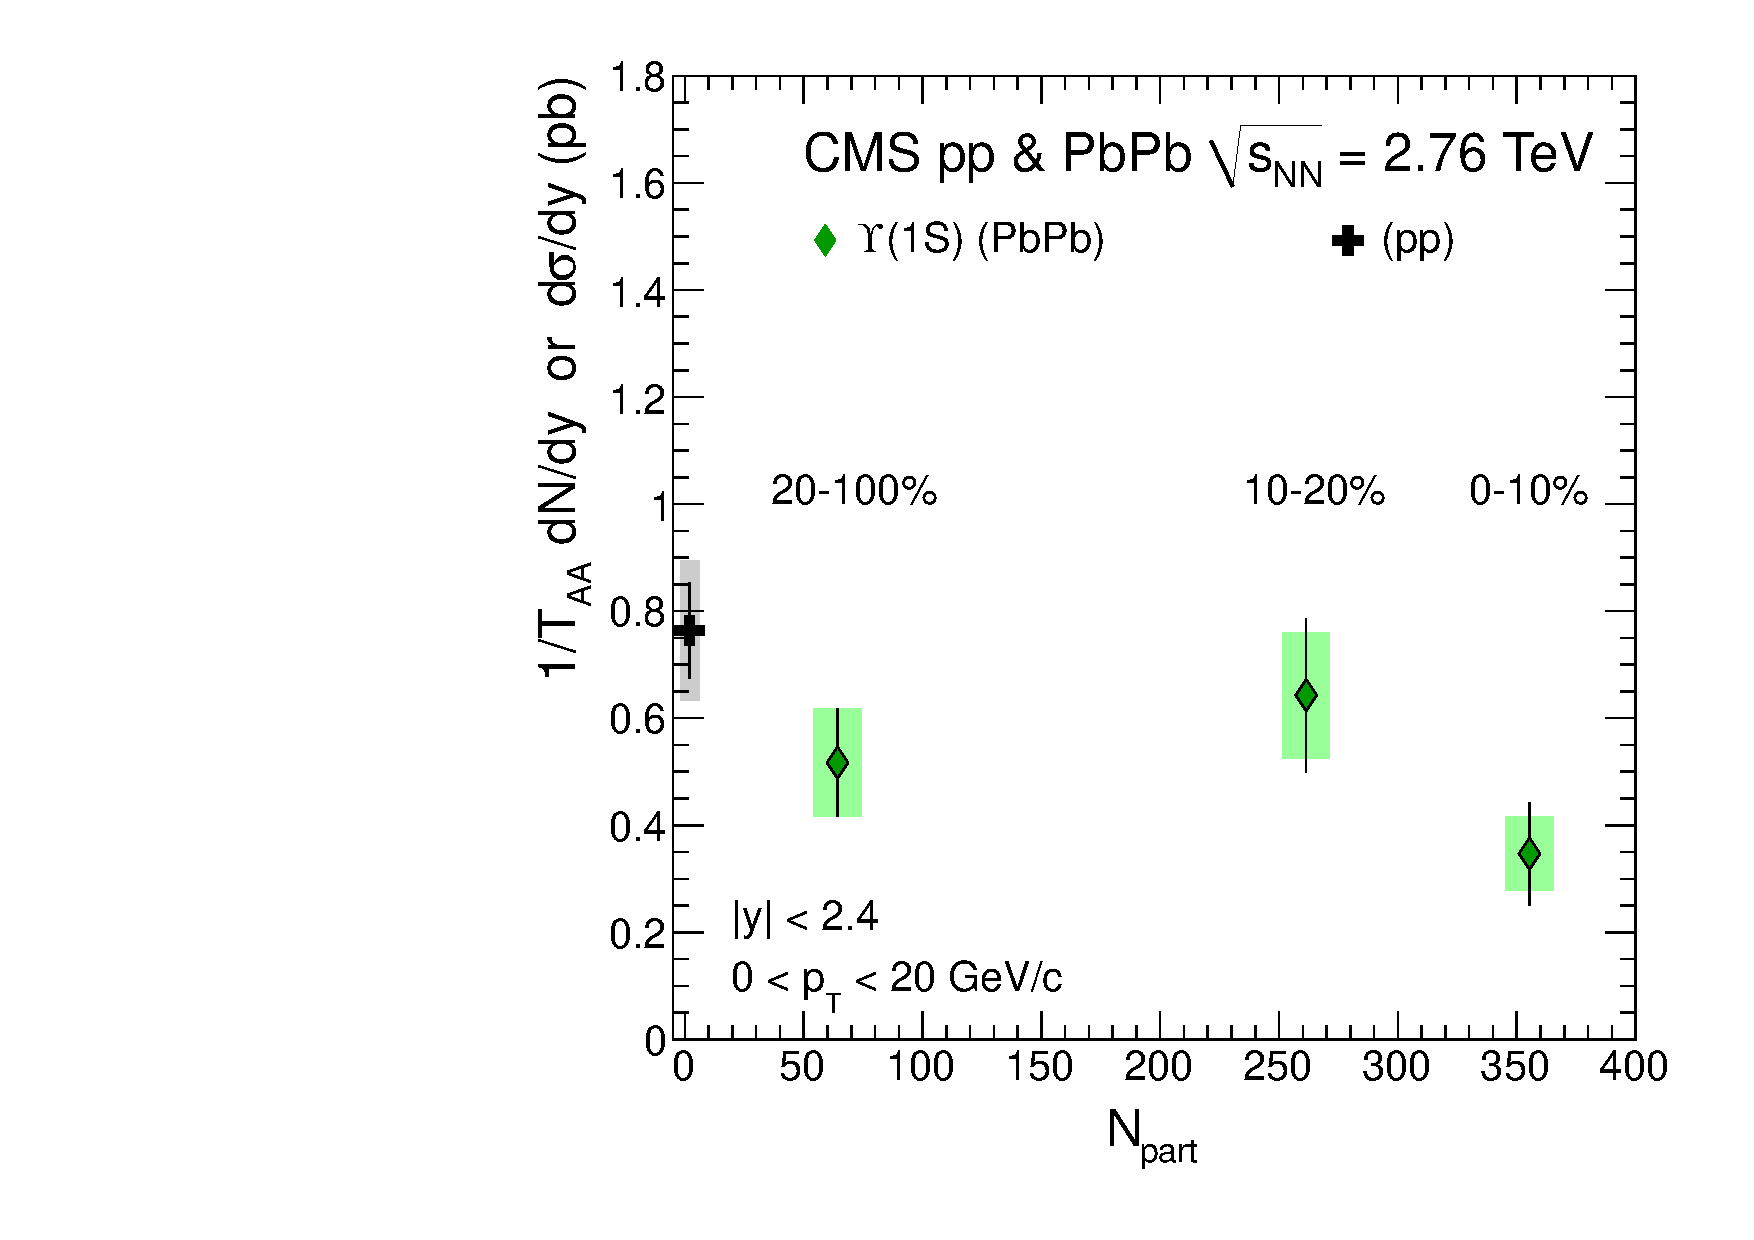
\includegraphics[width=0.45\textwidth]{chap_YInPbPbColl2010_figures/upsilon_cent}\hspace{1em}
    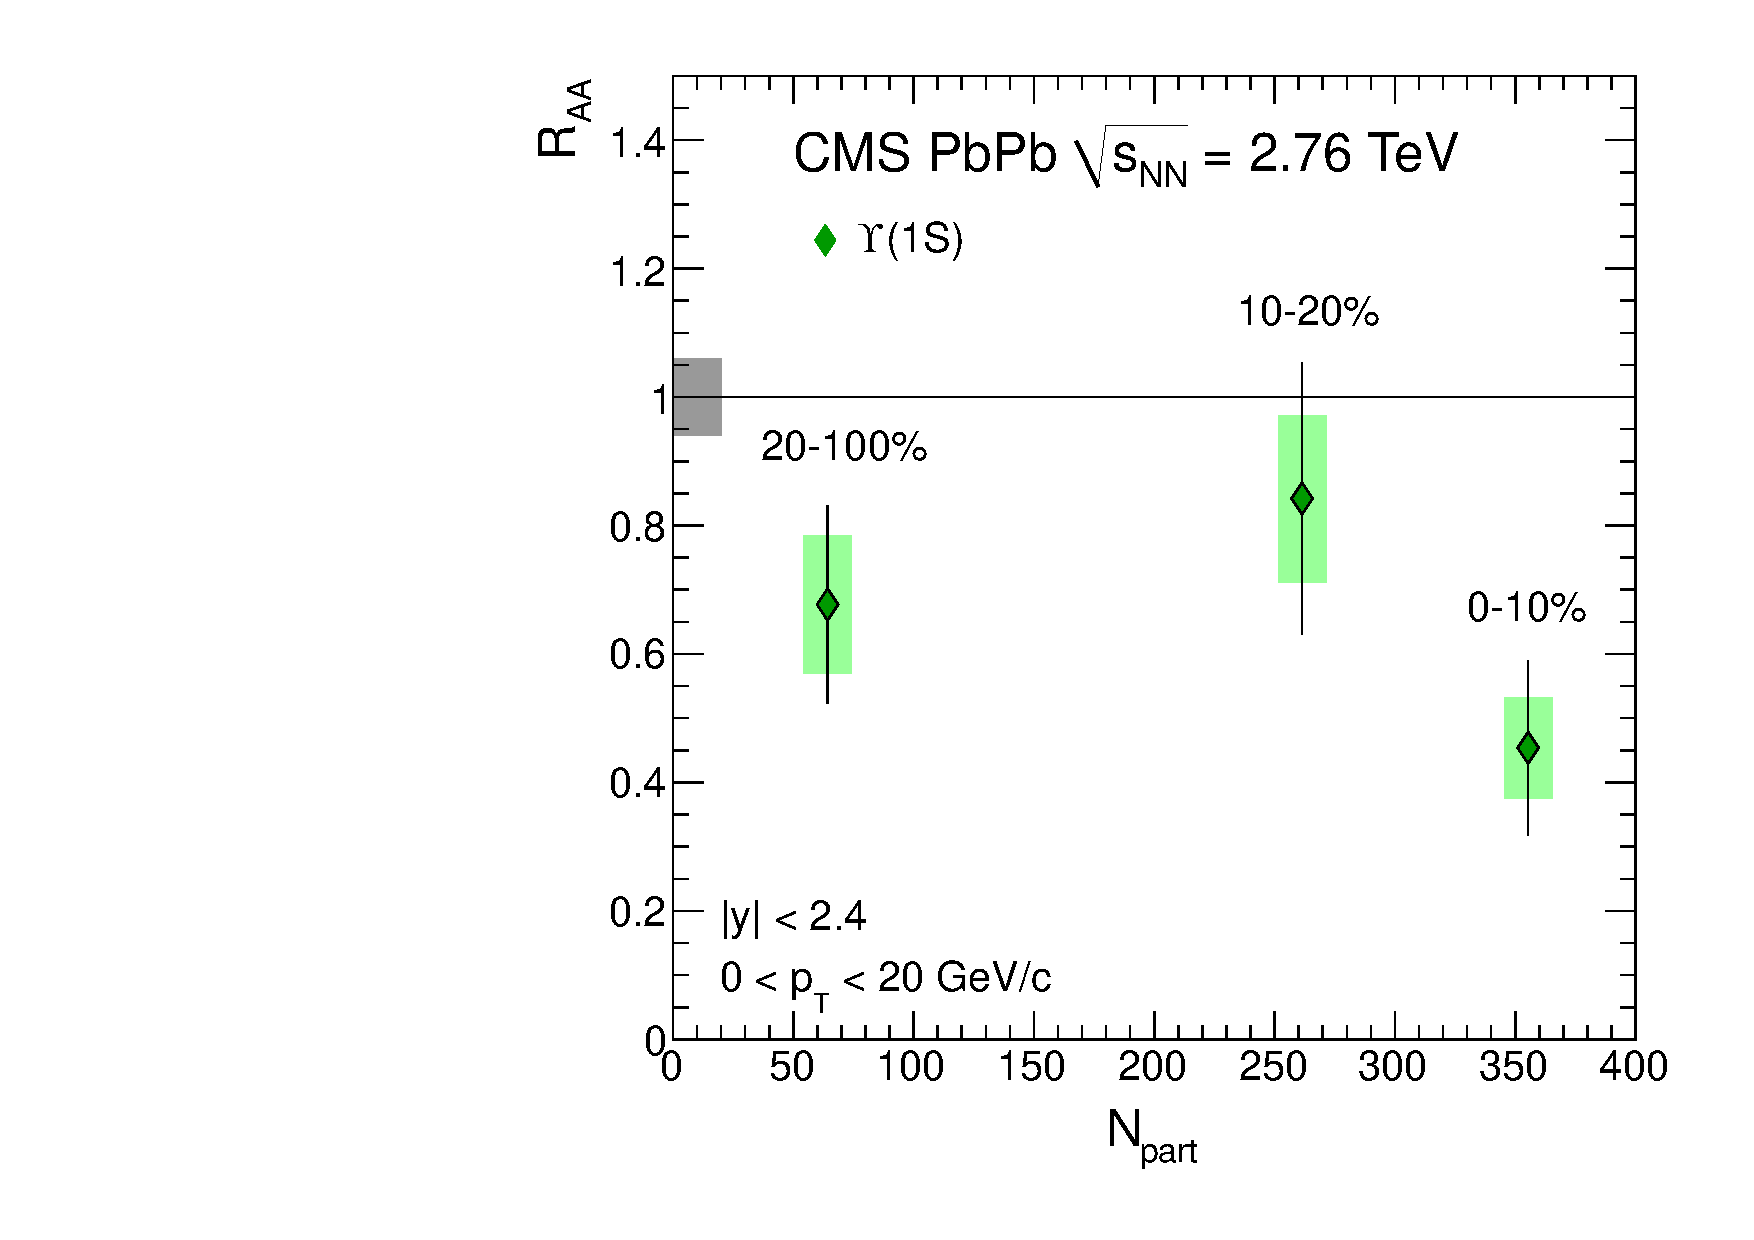
\includegraphics[width=0.45\textwidth]{chap_YInPbPbColl2010_figures/upsilon_RAA.pdf}
    \caption{Left: \PgUa\ yield divided by \taa (green diamonds) as a
      function of \npart compared to the \PgUa\ cross section measured
      in \pp (black cross). Right: nuclear modification factor \raa of
      \PgUa\ as a function of \npart. A global uncertainty of 6\%, from
      the integrated luminosity of the \pp data sample, is shown as a
      grey box at $\raa=1$. Statistical (systematic) uncertainties are
      shown as bars (boxes).}
    \label{fig:upsilon_cent}
  \end{center}
\end{figure}


\section{Indication of suppression of excited $\Upsilon$ states in PbPb collisions at $\sqrt{s_{\rm NN}} = 2.76$~TeV}
\label{sec:YDoubleRatio2010}
A comparison of the relative yields of $\Upsilon$ resonances in the $\mu^+\mu^-$ decay channel in PbPb and pp collisions at a centre-of-mass energy per nucleon pair 
of 2.76~TeV, is performed with data collected with the CMS detector at the LHC. Using muons of transverse momentum above 4~GeV/$c$ and pseudorapidity below 2.4, 
the double ratio of the $\Upsilon(2S)$ and $\Upsilon(3S)$ excited states to the $\Upsilon(1S)$ ground state in PbPb and pp collisions, 
$[\Upsilon(2S+3S)/\Upsilon(1S)]_{\rm PbPb} / [\Upsilon(2S+3S)/\Upsilon(1S)]_{\Pp\Pp}$, is found to be 0.31~$_{-0.15}^{+0.19}$~(stat.)~$\pm$~0.03~(syst.). 
The probability to obtain the measured value, or lower, if the true double ratio is unity, is calculated to be less than 1\%.
The measurement is performed with the data recorded by the Compact Muon Solenoid (CMS) experiment during the first PbPb LHC run, at the end of 2010, and during the 
pp run of March 2011, both at $\sqrt{s_{\rm NN}} = 2.76$~TeV. The integrated luminosity used in this analysis corresponds to 7.28~$\mu$b$^{-1}$ for PbPb and 
225~nb$^{-1}$ for pp collisions, the latter corresponding approximately to the equivalent nucleon-nucleon luminosity of the PbPb run. 
The excellent momentum resolution of the CMS detector results in well-resolved $\Upsilon$ peaks in the dimuon mass spectrum. 

A detailed description of the CMS detector can be found in~\ref{sec:YDoubleRatio2010}. Its central feature is a superconducting solenoid of 6~m internal diameter, 
providing a magnetic field of 3.8~T. Within the field volume are the silicon pixel and strip tracker, the crystal electromagnetic calorimeter, and the 
brass/scintillator hadron calorimeter. Muons are measured in gas-ionisation detectors embedded in the steel return yoke. In addition, 
CMS has extensive forward calorimetry, in particular two steel/quartz-fiber Cerenkov hadron forward (HF) calorimeters, which cover the pseudorapidity 
range $2.9 < |\eta| < 5.2$.

In this analysis, $\Upsilon$ mesons are identified through their dimuon decay. The silicon pixel and strip tracker measures charged-particle 
trajectories in the  range $|\eta| < 2.5$. The tracker consists of 66M pixel and 10M strip detector channels, providing a vertex resolution of 
$\sim$\,15~$\mu$m in the transverse plane. Muons are detected in the $|\eta| < 2.4$ range, with detection planes based on three technologies: 
drift tubes, cathode strip chambers, and resistive plate chambers. Due to the strong magnetic field and the fine granularity of the silicon tracker, 
the muon transverse momentum measurement ($p_{\rm T}$) based on information from the silicon tracker alone has a resolution between 
1 and 2$\%$ for a typical muon in this analysis.

In both the PbPb and pp runs, the events are selected by the CMS two-level trigger. At the first, hardware level, two independent muon candidates are 
required in the muon detectors. No selection is made on momentum or pseudorapidity, but in the pp case more stringent quality requirements are imposed 
for each muon in order to reduce the higher trigger rate. In both cases, the software-based higher-level trigger accepts the lower-level decision without 
applying further criteria. From reconstructed $J/\psi \rightarrow \mu\mu$ decays, the single-muon trigger efficiencies are measured and found to be consistent 
between the PbPb, $(96.1 \pm 1.0)\%$, and the pp, $(95.5 \pm 0.6)\%$, data sets, for muons with $p_{\rm T} >$~4~GeV/$c$.

In the PbPb data, events are preselected offline if they contain a reconstructed primary vertex made of at least two tracks, and a coincidence in both 
HF calorimeters of energy deposits in at least three towers of 3~GeV each. These criteria reduce contributions from single-beam interactions 
(e.g. beam-gas and beam-halo collisions with the beam pipe), ultra-peripheral electromagnetic collisions, and cosmic-ray muons. A small fraction of 
the most peripheral PbPb collisions is not selected by these requirements, which accept $(97 \pm 3)$\% of the hadronic inelastic 
cross section. For the pp run, a similar event filter is applied, relaxing the HF coincidence to one tower in each HF, with at least 3~GeV deposited. 
This filter removes only 1$\%$ of the pp events satisfying the dimuon trigger.

The muon offline reconstruction is seeded with $\simeq 99\%$ efficiency by tracks in the muon detectors, called standalone muons. 
These tracks are then matched to tracks reconstructed in the silicon tracker by means of an algorithm optimised for the 
heavy-ion environment~\cite{Roland:2006kz,D'Enterria:2007xr}. For muons from $\Upsilon$ decays the tracking efficiency is $\simeq$~85\%. 
This efficiency is lower than in pp, as in PbPb the track reconstruction is seeded by a greater number of pixel hits to reduce the large number 
of random combinations arising from the high multiplicity of each event. Combined fits of the muon and tracker tracks are used to obtain the 
results presented in this section. The heavy-ion dedicated reconstruction algorithm is applied to the pp data in order to avoid potential biases, 
arising from different tracking efficiencies of the two reconstruction algorithms, when comparing the two data sets.

Identical very loose selection criteria are applied to the muons in the pp and PbPb data. The transverse (longitudinal) distance from the event 
vertex is required to be less than 3 (15) cm. Tracks are only kept if they have 11 or more hits in the silicon tracker and the $\chi^2$ per degree 
of freedom of the combined (tracker) track fit is lower than 20 (4). The two muon trajectories are fit with a common vertex constraint, 
and events are retained if the fit $\chi^2$ probability is larger than 1$\%$. This removes background arising primarily from displaced heavy 
quark semileptonic decays. As determined from Monte Carlo simulation of the $\Upsilon(1S)$ signal, these selection criteria are found to 
reduce the efficiency by 3.9$\%$, consistent with the signal loss observed in both pp and PbPb data. The available event sample limits to 
20~GeV/$c$ the dimuon transverse momentum range probed in this study.

In order to further reduce the background in the $\Upsilon$ mass region, only muons with a transverse momentum ($p_{\rm T}^\mu$) higher than 
4~GeV/$c$ are considered, resulting in a $\Upsilon$ acceptance of approximately 25$\%$  for the $|y^\Upsilon|<2.4$ rapidity range. This 
requirement improves the significance of the $\Upsilon(1S)$ signal in PbPb data and is applied to both data sets. The acceptance of 
a $\Upsilon$ state depends on its mass, since the excited states give rise to higher-momenta muons. In consequence, requiring higher 
$p_{\rm T}^\mu$ increases the acceptance for the excited states relative to the ground state. 
In the corresponding analysis performed with the higher-statistics (3.1~pb$^{-1}$) 7~TeV data~\cite{Khachatryan:2010zg}, looser criteria were applied 
($p_{\rm T}^\mu >$~3.5 GeV/$c$ and $|\eta^\mu| < 1.6$, or $p_{\rm T}^\mu >$2.5 GeV/$c$ and $1.6 < |\eta^\mu| < 2.4$), where $\eta^\mu$ is the muon pseudorapidity. 
The stricter ($p_{\rm T}^\mu >$~4~GeV/$c$) requirements used here  enhance the  $\Upsilon(2S+3S)/\Upsilon(1S)$ yield ratio by $\simeq 60$\% in the \Pp\Pp\ data 
at 2.76~TeV. It was checked that, applying the same reconstruction algorithm and the same $p_{\rm T}^\mu$ requirements, the $\Upsilon(2S+3S)/\Upsilon(1S)$ yield 
ratio is consistent between the 2.76 and 7~TeV pp data sets.
The dimuon invariant mass spectra with the selection criteria applied are shown in Fig.~\ref{fig:massY2010} for the pp and PbPb data sets. Within the 7--14~GeV/$c^2$ 
mass range, there are 561 (628) opposite-sign muon pairs in the pp (PbPb) data set. The three Y peaks are clearly observed in the pp case, but the 
$\Upsilon(2S)$ and $\Upsilon(3S)$ are barely visible over the residual background in PbPb collisions.

\begin{figure}[hbtp]
  \begin{center}
    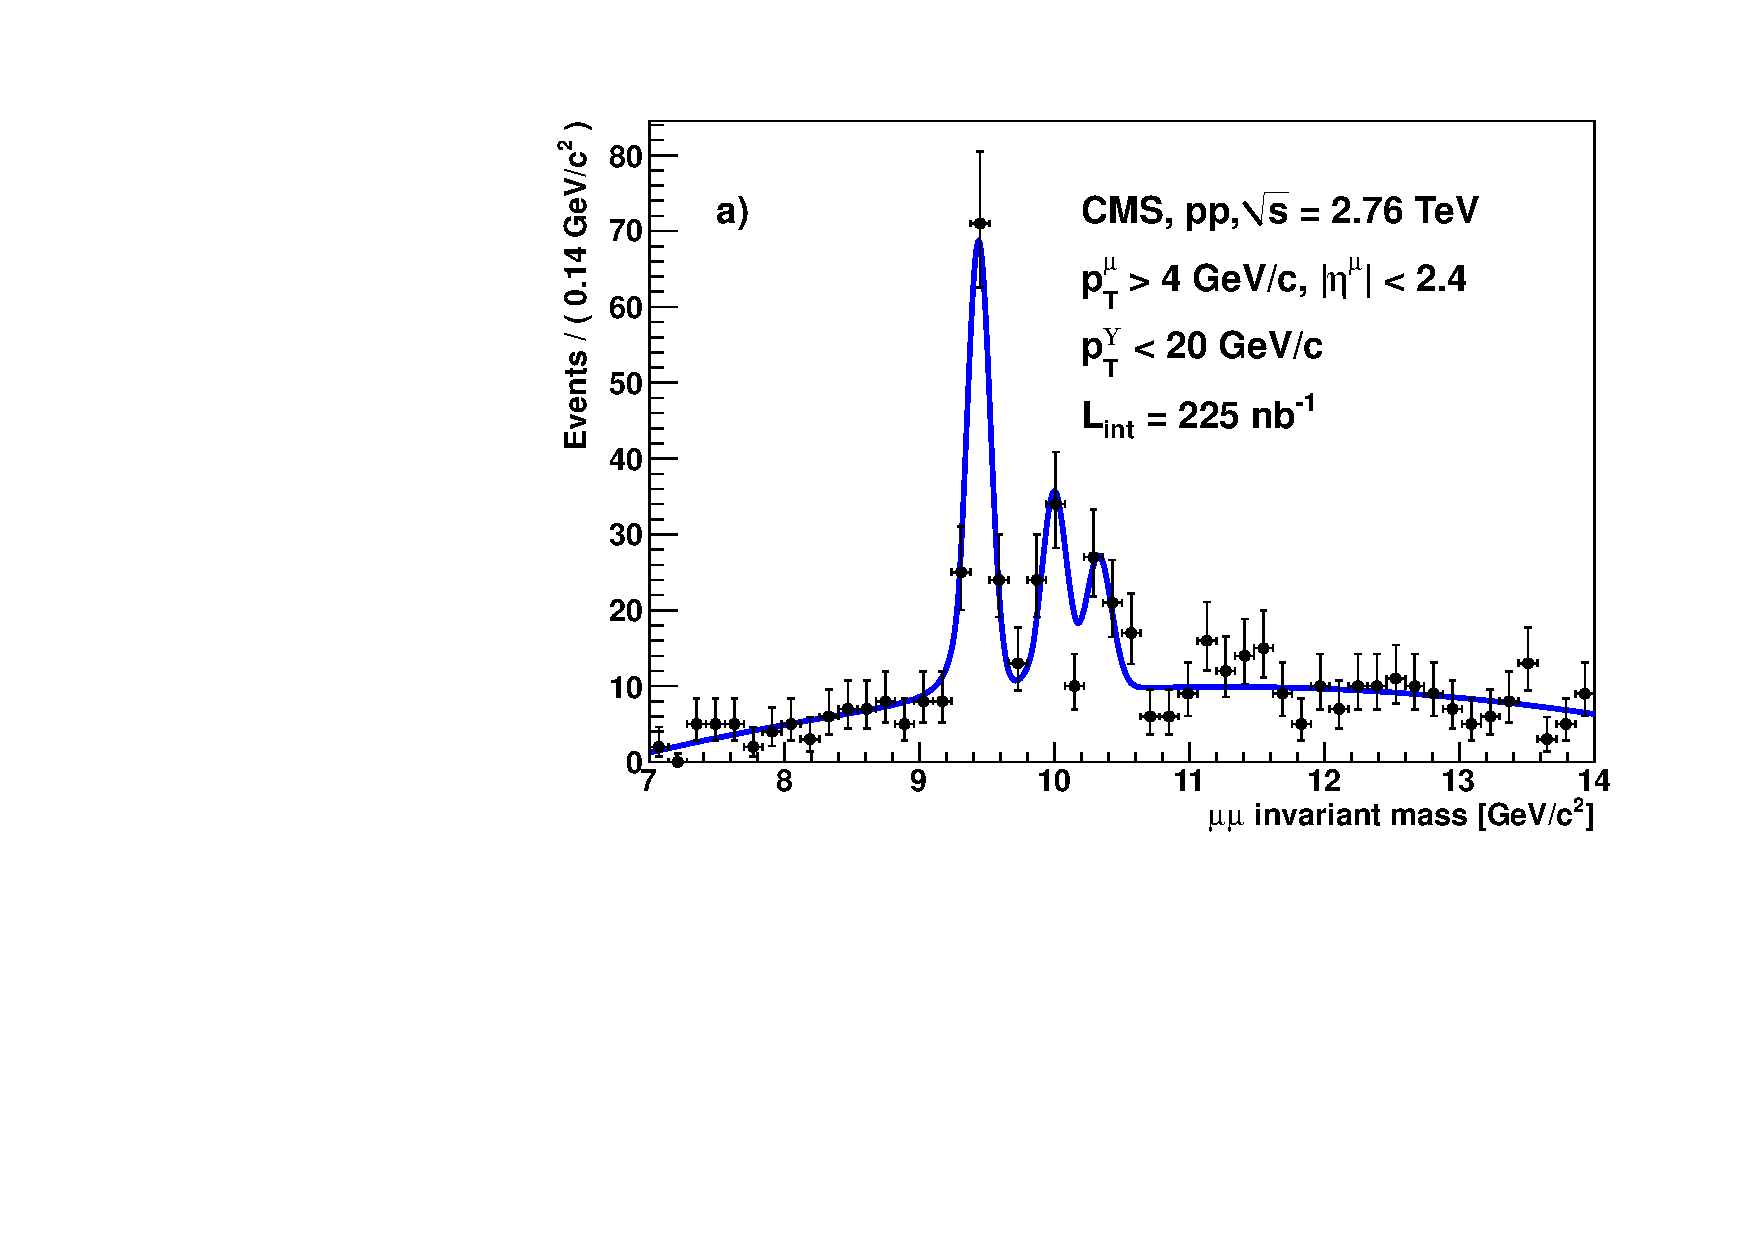
\includegraphics[width=0.95\linewidth]{chap_YInPbPbColl2010_figures/Mass_pp.pdf} 
    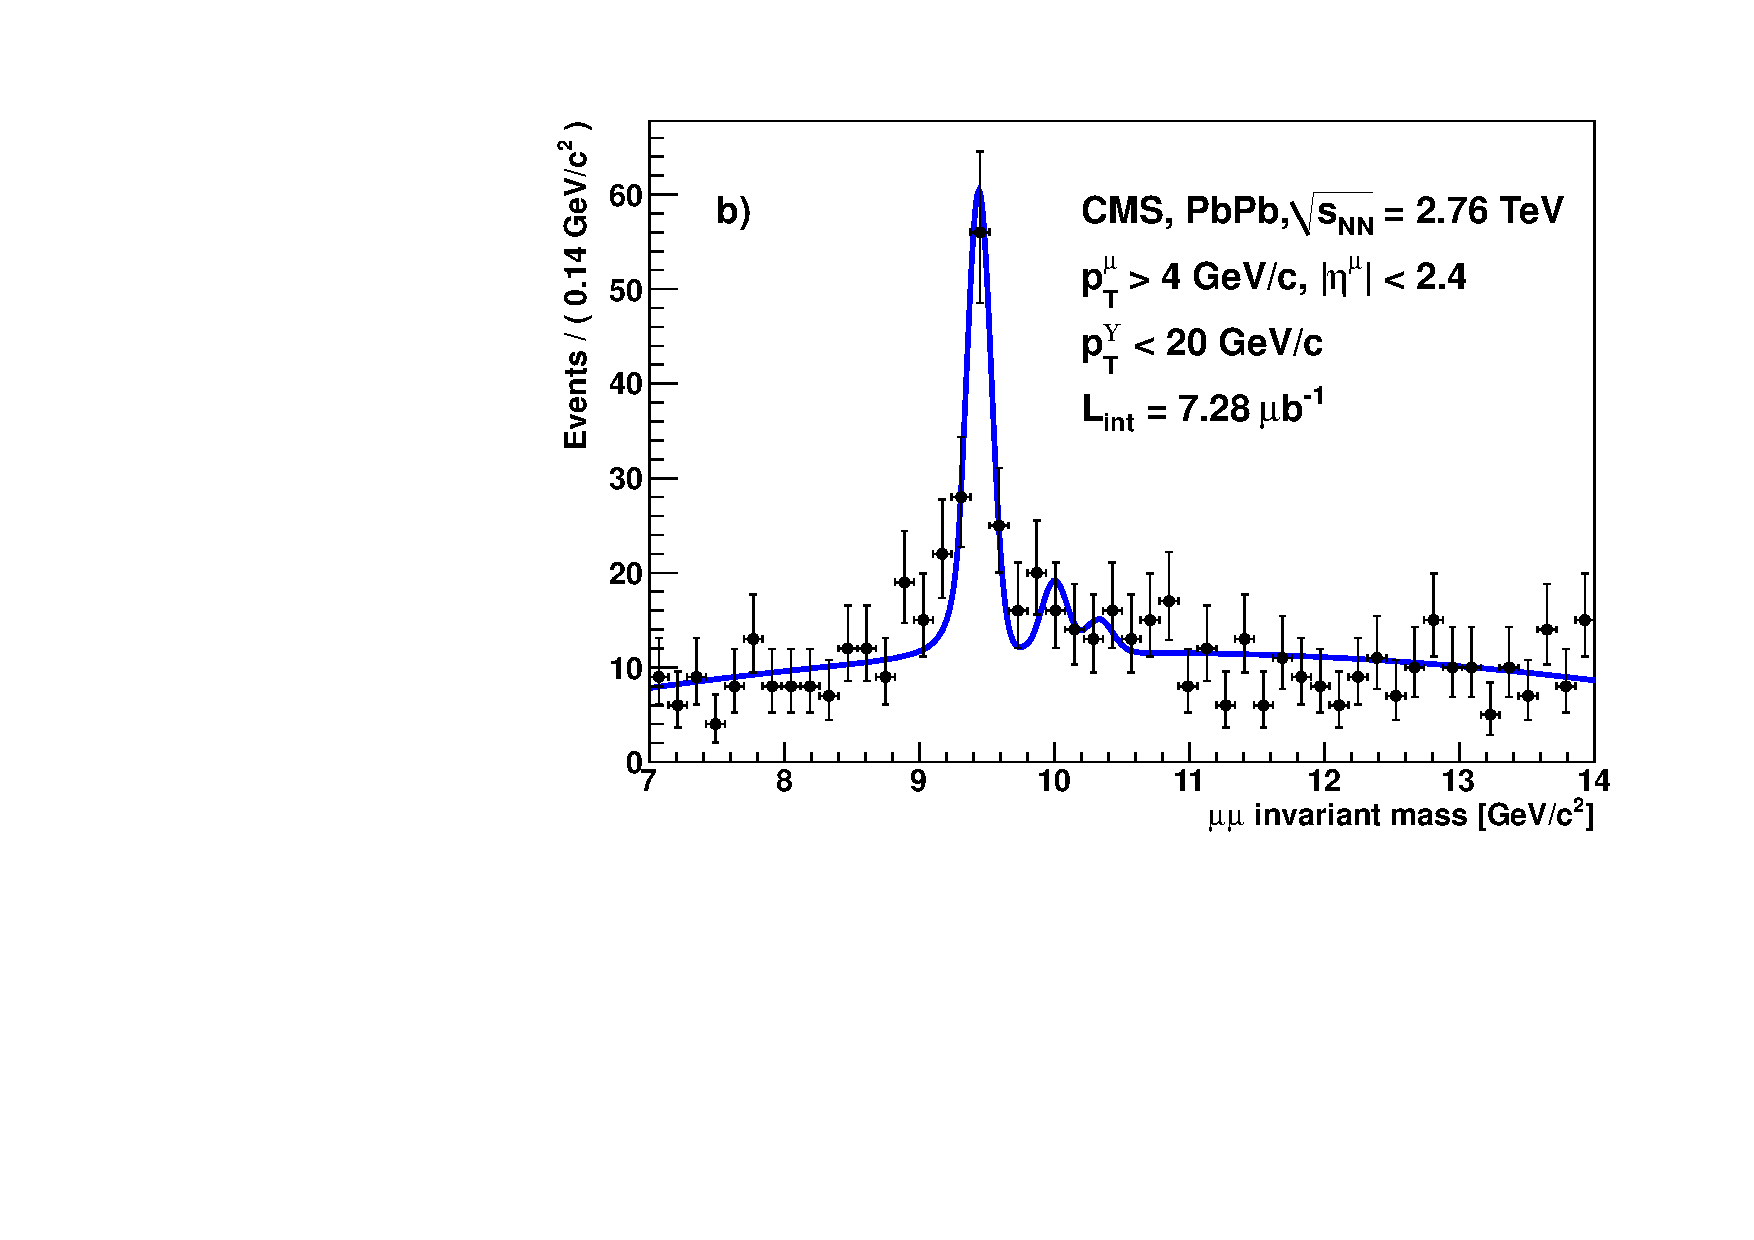
\includegraphics[width=0.95\linewidth]{chap_YInPbPbColl2010_figures/Mass_PbPb_nofit.pdf} 
    \caption{Dimuon invariant-mass distributions from the \Pp\Pp\ (a) and PbPb (b) data at $\sqrt{s_{\rm NN}} = 2.76$~TeV. 
      The same reconstruction algorithm and analysis criteria are applied to both data sets, including a transverse momentum requirement on 
      single muons of $p_{\rm T}^\mu >$~4~GeV/$c$. The solid lines show the result of the fit described in the text.}
    \label{fig:massY2010}
  \end{center}
    \vspace{-2ex}
\end{figure}
An extended unbinned maximum likelihood fit to the two invariant mass distributions of Fig.~\ref{fig:mass} is performed to extract the yields, following the 
method described in~\cite{Khachatryan:2010zg}. The measured mass lineshape of each $\Upsilon$ state is parameterised by a ``Crystal Ball'' (CB) function, i.e. 
a Gaussian resolution function with the low-side tail replaced by a power law describing final state radiation (FSR). Since the three $\Upsilon$ resonances partially 
overlap in the measured dimuon mass, they are fit simultaneously. Therefore, the probability distribution function (PDF) describing the signal consists of three CB 
functions. In addition to the three $\Upsilon(nS)$ yields, the $\Upsilon(1S)$ mass is the only parameter left free, to accommodate a possible bias in the momentum 
scale calibration. The mass differences between the states are fixed to their world average values~\cite{Nakamura:2010zzi} and the mass resolution is forced to scale 
with the resonance mass. The $\Upsilon(1S)$ resolution is fixed to the value estimated in the simulation, 92~MeV/$c^2$, which is compatible with the resolution obtained 
from both the PbPb and pp data. The low-side tail parameters are also fixed to the values obtained via simulation. Finally, a second-order polynomial is chosen to 
describe the background in the 7--14~GeV/$c^2$ mass-fit range.
The quality of the unbinned fit is checked \emph{a posteriori} by comparing the obtained lineshapes to the binned data of Fig.~\ref{fig:massY2010}. 
The $\chi^2$ probabilities are 74$\%$ and 77$\%$, respectively for pp and PbPb.

The ratios of the observed yields of the $\Upsilon(2S)$ and $\Upsilon(3S)$ excited states to the $\Upsilon(1S)$ ground state in the pp and PbPb data are:
\begin{eqnarray}
  \Upsilon(2S+3S)/\Upsilon(1S)|_{\Pp\Pp} & = & 0.78 _{-0.14}^{+0.16} \pm 0.02,\\
  \Upsilon(2S+3S)/\Upsilon(1S)|_{\rm PbPb} & = & 0.24 _{-0.12}^{+0.13} \pm 0.02,
\end{eqnarray}
where the first uncertainty is statistical and the second is systematic.

The systematic uncertainties are computed by varying the lineshape in the following ways: 
\begin{enumerate}
\item the CB-tail parameters are varied randomly according to their covariance matrix and within conservative values covering imperfect 
knowledge of the amount of detector material and FSR in the underlying process; 

\item the resolution is varied by $\pm 5$~MeV/$c^2$, which is a conservative variation given the current understanding of the detector performance 
and reasonable changes that can be anticipated in the $\Upsilon$-resonance kinematics between pp and PbPb data; 

\item the background shape is changed from quadratic to linear while the mass range of the fit is varied from 6--15 to 8--12~GeV/$c^2$; 
\end{enumerate}
the observed root-mean-square of the results is taken as the systematic uncertainty. The quadrature sum of these three systematic uncertainties 
gives a relative uncertainty on the ratio of 10$\%$ (3$\%$) on the PbPb (pp) data.

The ratio of the $\Upsilon(2S+3S)/\Upsilon(1S)$ ratios in PbPb and pp benefits from an almost complete cancellation of possible acceptance 
and/or efficiency differences among the reconstructed resonances. A simultaneous fit to the pp and PbPb mass spectra gives the double ratio
\begin{equation}
  \frac{\Upsilon(2S+3S)/\Upsilon(1S)|_{\rm PbPb}}{\Upsilon(2S+3S)/\Upsilon(1S)|_{\Pp\Pp}}
 = 0.31 _{-0.15}^{+0.19} \; ({\rm stat.}) \pm 0.03 \; ({\rm syst.}),
\label{eq:double}
\end{equation}
where the systematic uncertainty (9$\%$) arises from varying the lineshape as described above in the simultaneous fit, 
thus taking into account partial cancellations of systematic effects.

To evaluate possible imperfect cancellations of acceptance and efficiency effects in the double ratio, a full GEANT4~\cite{Agostinelli:2002hh} detector 
simulation is performed. The effect of the higher PbPb underlying event activity is considered by embedding, at the level of detector signals, $\Upsilon(1S)$ 
and $\Upsilon(2S)$ decays simulated by PYTHIA 6.424~\cite{Sjostrand:2006za} in PbPb events simulated with \textsc{hydjet}~\cite{Lokhtin:2005px}. 
Track characteristics, such as the number of hits and the $\chi^2$ of the track fit, have similar distributions in data and simulation. As mentioned above, the 
trigger efficiency is evaluated with data, by using single-muon-triggered data events, and reconstructing J/$\psi$ signal with and without the dimuon trigger requirement. 
The same exercise is carried out with the simulation and it agrees with the efficiency measured in data at the 2$\%$ level. The track efficiency in the silicon detector 
is measured with standalone muons, applying all selection criteria. The efficiencies in data and simulation agree within the 4$\%$ statistical uncertainty of the 
efficiency determined from data.
The difference in reconstruction and selection efficiencies between the $\Upsilon$ states is less than 5$\%$ and the variation with charged particle multiplicity is less 
than 10$\%$ from pp to central PbPb collisions, producing a maximum change of 0.5$\%$ on the double ratio. The good agreement between single-muon trigger efficiencies 
extracted from data for the pp and PbPb trigger requirements, applied to the $\Upsilon(1S)$ and $\Upsilon(2S)$ trigger efficiencies derived from simulation, leads to a 
negligible effect on the double ratio. The single-muon trigger efficiencies extracted from data agree within 1.5$\%$ for the pp and PbPb trigger requirements, and the 
$\Upsilon(1S)$ and $\Upsilon(2S)$ trigger efficiencies agree within 3$\%$, according to simulation: the potential trigger bias on the double ratio is negligible. 
The magnitudes of the statistical and systematic uncertainties on the double ratio, respectively 55$\%$ and 9$\%$, are significantly larger than the systematic 
uncertainties associated with possible imperfect cancellation of acceptance and efficiency effects. Therefore no additional uncertainty from these sources is applied.
Finally, using an ensemble of one million pseudo-experiments, generated with the signal lineshape obtained from the pp data (Fig.~\ref{fig:massY2010}a), the background 
lineshapes from both data sets, and a double ratio (Eq.~\ref{eq:double}) equal to unity within uncertainties, the probability of finding the measured value of 0.31 or 
below is estimated to be 0.9$\%$. In other words, in the absence of a suppression due to physics mechanisms, the probability of a downward departure of the ratio from 
unity of this significance or greater is 0.9$\%$, i.e. that corresponding to 2.4 sigma in a one-tailed integral of a Gaussian distribution.
Studies in section \ref{sec:results} show that the $\Upsilon(1S)$ itself is suppressed by about 40$\%$ in minimum bias PbPb collisions at 
$\sqrt{s_{\rm NN}} = 2.76$~TeV. Since a large fraction of the $\Upsilon(1S)$ yield arises from decays of heavier bottomonium states~\cite{Affolder:1999wm}, 
this $\Upsilon(1S)$ suppression could be indirectly caused by the suppression of the excited states.

Production yields of quarkonium states can also be modified, from pp to PbPb collisions, in the absence of QGP formation, by cold nuclear matter effects~\cite{Vogt:2010aa}. 
However, such effects should have a small impact on the $\Upsilon$ double ratio reported here. The nuclear modifications of the parton distribution functions (shadowing) 
should have an equivalent effect on the three $\Upsilon$ states, because their production involves very similar partons, cancelling in the ratio, at least to first order. 
The same should happen to any other initial-state nuclear effect. In principle, the larger and more loosely bound excited quarkonium states are more likely to be broken 
up by final-state interactions while traversing the nuclear matter, something extensively studied in the context of charmonium suppression at lower energies
~\cite{Lourenco:2008sk}. 
This ``nuclear absorption'' becomes weaker with increasing energy, and should be negligible at the LHC. At RHIC energies, the STAR experiment~\cite{Reed:2011zz} has reported 
a $\Upsilon(1S+2S+3S)$ yield in dAu collisions of $0.78 \pm 0.28 \pm 0.20$ times the yield expected by scaling pp collisions, compatible with the absence of absorption. 
Furthermore, the double ratio presented here would only be sensitive to a \emph{difference} between the nuclear dependencies of the three states and already at much lower energies 
the Fermilab E772 experiment observed~\cite{Alde:1991sw}, in proton-nucleus collisions, no such difference, within uncertainties, between the $\Upsilon(1S)$ and 
the sum $\Upsilon(2S+3S)$.





\section{Discussion}
\label{sec:discussion}
The \PgUa\ yield divided by \taa as a function of \pt, rapidity, and
centrality has been measured in \PbPb collisions.  No strong
centrality dependence is observed within the uncertainties. The
nuclear modification factor integrated over centrality is $\raa =
0.63\pm0.11\,(\text{stat.})\pm0.09\,(\text{syst.})$. This suppression
is observed predominantly at low \pt. Using \ppbar collisions at
\sqrts = 1.8\TeV, CDF measured the fraction of directly produced \PgUa\
as $(50.9\pm8.2\,(\text{stat.})\pm9.0\,(\text{syst.}))\%$ for \PgUa\
with $\pt>8\GeVc$~\cite{Affolder:1999wm}. Therefore, the \PgUa\
suppression presented in this paper could be indirectly caused by the
suppression of excited \PgU\ states.
Comparison of the relative yields of $\Upsilon$ resonances has been performed in PbPb and pp collisions at the same 
centre-of-mass energy per nucleon pair of 2.76 TeV. The double ratio of the $\Upsilon(2S)$ and $\Upsilon(3S)$ excited states to the $\Upsilon(1S)$ 
ground state in PbPb and pp collisions, $[\Upsilon(2S+3S)/\Upsilon(1S)]_{\rm PbPb}/[\Upsilon(2S+3S)/\Upsilon(1S)]_{\Pp\Pp}$, is found to be 
0.31~$_{-0.15}^{+0.19}$~(stat.)~$\pm$~0.03~(syst.), for muons of $p_{\rm T}>4$~GeV/$c$ and $|\eta|<2.4$. 
The probability to obtain the measured value, or lower, if the true double ratio is unity, has been calculated to be less than 1\%. 

